\chapter{Dynamic Decision Trees}
\section{Introduction}
Decision trees are a cornerstone of machine learning, and an essential tool in any machine learning library. Decision-tree-based algorithms such as random forests or XGBoost, are widely used to solve real-world machine learning problems. They also boast the appealing feature of being explainable\todo{Add ref to papers about explainability of DT}.
As many other machine learning problems, the classification problem has a \define{dynamic} version, as explained in section \ref{subsec:dynamic_intro}. In that version the training dataset evolves with time by inserting and deleting data points. The dynamic classification problem is called \define{fully-dynamic} if insertions and deletions are permitted, and \define{online} or \define{incremental} if only the former applies.

In the online version, there is an additional difficulty called \define{concept drift}. Is that case, the underlying model that make data belong to one class or another change with time so that the relevance of the data is maximal at the time when they are inserted and slowly decay as new points are inserted. Thus if the model is updated by considering each data equally, its accuracy will be sharply reduced. If the algorithm used to build the model can handle the fully-dynamic problem, then it is possible to handle the concept drift by working on a window of data, i.e. setting a constant $t$ and only working on the last $t$ inserted data, deleting the oldest data each time a new one is inserted. There are however algorithms built specifically for the online problem that can handle concept drift.

Many variants of the Decision Tree method exist to deal with the online problem. However, to the best of our knowledge the only variant compatible with the fully-dynamic problem is BOAT\todo{Add citation}. This method however was not specifically designed for this task\todo{Add ref to discussion?}.

This chapter presents a new fully-dynamic decision tree building algorithm. We first review the literature related to online decision trees. The Gini gain theorem and a new target for fully-dynamic decision trees in then described, before detailing the algorithm. The following two sections present the theoretical and experimental results of our algorithms. Finally we discuss the findings and we conclude.

\subsection{Our contributions}
\subsection{Organisation of the chapter}
\subsection{Acknowledgements}

\section{Online decision trees: A brief review of the literature}
\todo{Redact this part}
 There is a rich literature for online decision tree algorithms (see~\cite{Manapragada2022_AnEagerSplitting} for a survey).
\begin{itemize}
    \item \cite{Domingos2000_HighSpeedStreams,Domingos2001_MiningTimeSeries,Gama2003_HighSpeedStreams,Jin2003_EfficientDecisionTree,Rutkowski2013_DecisionTreesForMining}: classic papers using concentration bounds to build near-optimal trees over streams
    \item \cite{Manapragada2018_EFDT}: introduces the Hoeffding Anytime Tree and its implementation EFDT (Extremely Fast Decision Tree)
    \item \cite{Das2019_LearnSmartWithLess}: improves on VFDT's conservativeness via statistical resampling
   \item \cite{sun2020_SpeedingUpVeryFast}: improves on VFDT by heuristically reducing the attempts and/or time to split 
   \item \cite{Barddal2020_RegularizedAndIncremental}: adds regularization to EFDT and others, to avoid too large trees
   \item \cite{Manapragada2022_AnEagerSplitting}: thorough study of the Hoeffding AnyTime Tree (EFDT) in ensemble setting, uses ``the largest and most comprehensive set of testbenches in the online learning literature''
   \item \cite{Haug2022_DynamicModelTree}: some other method called ``Dynamic Model Tree'' which is claimed to outperform previous methods
\end{itemize}

%There have been increasing efforts in recent years in developing fully dynamic algorithms for machine learning problems, with most of the literature focusing on unsupervised tasks, such as clustering~\cite{Cohen-Addad2019_FullyDynamicConsistent, Henzinger2020_FullyDynamicCoresets, Bateni2021_OptimalFullyDynamic, Chan2018_FullyDynamicKCenter}, graph mining~\cite{Bhattacharya2015_SpaceAndTimeEfficientAlgorithm, Epasto2015_EfficientDensestSubgraph, DeStefani2017_TRIESTCountingLocal} and other optimization problems~\cite{DBLP:conf/nips/LattanziMNTZ20, DBLP:journals/siamcomp/BhattacharyaHI18}.
%However, to the best of our knowledge, fully-dynamic supervised machine learning has been mostly unexplored so far. 
%The works closest to ours are those in the incremental setting. Here, the algorithm receives a stream of examples from a distribution, and has to perform well when compared to the offline tree built on the entire sequence. In this setting, Hoeffding trees~\cite{Domingos2000_HighSpeedStreams} emerged as one of the most effective approaches, inspiring several variants, even ones capable of handling concept drifts~\cite{Domingos2001_MiningTimeSeries,Gama2003_HighSpeedStreams,Manapragada2018_EFDT,Das2019_LearnSmartWithLess,sun2020_SpeedingUpVeryFast,Haug2022_DynamicModelTree,Jin2003_EfficientDecisionTree,Rutkowski2013_DecisionTreesForMining}; see~\cite{Manapragada2022_AnEagerSplitting} for a survey. These algorithms crucially rely on the examples being i.i.d., which allows them to compute good splits with high probability via concentration bounds (whence the name). Moreover, those algorithms cannot handle efficiently real-valued features, since on those features they would update $\Theta(n)$ counters at each time, even when only insertions are allowed. Our algorithms instead efficiently handle arbitrary sequences of insertions and deletions of examples with real-valued features. 
\section{Preliminaries}
\subsection{Gini index and Gini gain smoothness}
The Gini index and Gini gain were introduced in section \ref{subsec:intro_dt_split_criteria}. The Gini gain is one of the main metrics used for determining the best splits in decision trees. We want to study to which extend a limited number of modifications to the training set can change the Gini index or the best Gini gain from the set. 

We use the following notation with $o$ a boolean operation:
\begin{equation}
    \delta_o = \begin{cases}
        1 & \text{ if $o$ is \codetrue}\\
        0 & \text{ else}
    \end{cases}
\end{equation}
We then have the following equivalent definition of the Gini index:
\begin{property}
    \begin{equation}\label{eq:gini_index_as_sum}
        g(S) = \frac{2}{n^2} \sum_{i=1}^{|S|}\sum_{j=i+1}^{|S|} \delta_{y_i \neq y_j}
    \end{equation}
\end{property}
\begin{proof}
    We have $\sum_{i=1}^{|S|}\sum_{j=1}^{|S|} \delta_{y_i = y_j} = \sum_{y \in \scY} N_{S,y}^2$. From equation \ref{eq:general_gini_index_def} we have:
    \begin{equation*}
        \begin{split}
            & g(S) = 1 - \frac{1}{n^2} \sum_{i=1}^{|S|}\sum_{j=1}^{|S|} \delta_{y_i = y_j}\\
            \Leftrightarrow & g(S) = \frac{1}{n^2} \sum_{i=1}^{|S|}\sum_{j=1}^{|S|} 1 - \delta_{y_i = y_j}
        \end{split}
    \end{equation*}
    We know that $1 - \delta_{y_i = y_j} = \delta_{y_i \neq y_j}$. We rearrange the terms to find the sum in equation \ref{eq:gini_index_as_sum} and conclude the proof.
\end{proof}

We call \define{edit distance} $\ED(S, S')$ from one set of data $S$ to another $S'$ the minimal number of insertions and deletions needed to build $S'$ from $S$. We first establish two lemma on the local smoothness of the Gini index and the Gini gain:
\begin{lemma}\label{lem:local_gini_index_smoothness}
    Let $S, S'$ be two set of training data of size at least 1. If $\ED(S, S') \leq 1$. then $|g(S) - g(S')| \leq \frac{2}{\max(|S|, |S'|)}$
\end{lemma}

%For the second lemma, we note $G(S, j, t)$ the Gini gain of splitting the training set $S$ along the feature $j$ using the threshold or category $t$. It means that, if the feature $j$ is numerical, the data points for which the feature $j$ is less than or equal to $t$ go to one subset while the other points go to the other subset. If the feature is categorical on the other hand, the data points that have the feature $j$ equals category $t$ go to one subset while the other points go to the other subset.
\begin{lemma}\label{lem:local_gini_gain_smoothness}
    Let $S, S'$ be two set of training data of size at least 1. Let $S_1$ and $S_2$ the two subsets created by a splitting function applied on $S$, and $S_1'$ and $S_2'$ the subsets created by the same splitting function applied on $S'$. If $\ED(S, S') \leq 1$. then
    \begin{equation*}
        |G(S, S_1, S_2) - G(S', S_1', S_2')| \leq \frac{12}{\max(|S|, |S'|)}        
    \end{equation*}
\end{lemma}

\begin{proof}[Proof of lemma \ref{lem:local_gini_index_smoothness}]
    The case $\ED(S, S') = 0$ is trivial, we assume $\ED(S, S') = 1$. Without loss of generality assume $S = \{(x_1, y_1)\} \cup S'$. Let $n = |S|$.
    
    Let $D_S = 2\sum_{i=1}^{|S|}\sum_{j=i+1}^{|S|} \delta_{y_i \neq y_j}$. We see that $g(S) = \frac{1}{n^2}D_S$. We also see that:
    \begin{equation*}
        D_S - 2(n-1) \leq D_{S'} \leq D_S
    \end{equation*}
    therefore we have:
    \begin{align}
        g(S') - g(S) &\geq \left(\frac{1}{(n-1)^2} - \frac{1}{n^2}\right)D_S - \frac{2}{n-1}\label{eq:proof_lem_loc_gini_ind_smooth_1}\\
        g(S') - g(S) &\leq \left(\frac{1}{(n-1)^2} - \frac{1}{n^2}\right)D_S\label{eq:proof_lem_loc_gini_ind_smooth_2}
    \end{align}
    We can factorize each inequation using $\frac{1}{(n-1)^2} - \frac{1}{n^2} = \frac{2n-1}{n^2(n-1)^2}$

    We first study (\ref{eq:proof_lem_loc_gini_ind_smooth_2}). We know that $D_S < (n-1)^2$, and so we have:
    \begin{equation*}
        g(S') - g(S) < \frac{2n-1}{n^2} < \frac{2}{n}
    \end{equation*}

    Now we study (\ref{eq:proof_lem_loc_gini_ind_smooth_1}). First note that if $D_S = 0$ then $g(S) = g(S') = 0$ and the theorem holds. We therefore focus on the case when $D_S > 0$.

    We note that if we consider the class $y$ that has the lowest number of data points, and we move one point from that class to another, then the value of $D_S$ is necessarily reduced or equal. From any training set $S$ st. $D_S > 0$ we can apply this process recursively to create a new training set $S^*$ of which all the points but one are in the same class. Since $D_{S^*} = 2(n-1)$ and the process only decreases $D_S$, we deduce that if $D_S > 0$ then $D_S \geq 2(n-1)$.

    Then, (\ref{eq:proof_lem_loc_gini_ind_smooth_1}) becomes:
    \begin{equation*}
        \begin{split}
            g(S') - g(S) &\geq \frac{2n-1}{n^2(n-1)^2} D_S - \frac{2}{n-1}\\
            &\geq 2\frac{2n-1}{n^2(n-1)} - \frac{2}{n-1}\\
            &\geq -\frac{2}{n}\left(\frac{n^2 - 2n + 1}{n (n-1)}\right)\\
            &\geq -\frac{2}{n}\left(\frac{n-1}{n}\right)\\
            &\geq -\frac{2}{n}
        \end{split}
    \end{equation*}
\end{proof}


We can now establish the following theorem:

\begin{theorem}
\label{th:smoothness}
Let $S,S'$ be sets of data.
\begin{enumerate}%\itemsep0pt
    \item $|G(S,j,t) - G(S',j,t)| \le 12 \EDR(S,S'), \forall (j,t) \in [d] \times \R$
    \item $|g(S)-g(S')| \le 2.5 \, \EDR(S,S')$.
\end{enumerate}
\end{theorem}
%If $S$ is a sequence of examples and $z$ is an example, then $S \cup \{x\}$ denotes the concatenation of $S$ and $x$, while $S \setminus \{z\}$ denotes the sequence obtained by deleting any one occurrence of $z$ from $S$. 

\subsection{$\beps$-feasibility: a new performance guarantee for dynamic decision trees}
\begin{definition}\label{def:eps_feasibility}
Let $k,h \in \N$, and let $\beps=(\epsThr,\epsApx)$ where $\epsThr,\epsApx \in (0, 1]$. A decision tree $(T,\Splits,L)$ is $\beps$-feasible, with pruning thresholds $(k,h)$, w.r.t.\ a multiset $S$ of labeled examples if for every $v \in V(T)$:
\begin{enumerate}
\item if $|S_v| \le k$ or $g(S_v) = 0$ or $\depth_T(v)=h$ then $v$ is a leaf, else if $g(S_v) \ge \epsThr$ then $v$ is an internal node
\item if $\sigma_v = (j,a)$ then $G(S_v,j,a) \geq G(S_v,j',a') - \epsApx$ for all $(j',a') \in [d] \times \R$
\item if $v$ is a leaf then $L_v$ is a majority label of $S_v$
\end{enumerate}
\end{definition}
For any fixed pruning thresholds $k,h$ we say that a fully dynamic algorithm $\scA$ is $\beps$-feasible if, at any point in time, $\scA$ is coherent with a decision tree $(T,\Splits,L)$ that is $\beps$-feasible with respect to the current active set. 
%\begin{theorem}[\textbf{OLD VERSION}]
%Fix $\beps$. There is an $\beps$-feasible fully dynamic decision tree algorithm in the adaptive adversary model that, for every sequence of $\scT$ update requests, uses space $O(nd)$ and has amortized running time per update \mbox{$O\big((h+\log n) \cdot d \cdot \frac{(1+\epsilon)^2}{\epsilon} \cdot \min (h,\log_{1+\epsilon} (n))\big)$}, where $n = \max_{t=1}^{\scT} |S^{t}|$ and $\epsilon=f(\beps)$.
%\end{theorem}
When $k=1$ and $h=\infty$ and $\epsThr=\epsApx$, $\beps$-feasibility reduces to the following condition: if $g(S_v)=0$ then $v$ is a leaf, and if $g(S_v) \ge \epsThr$ then $v$ is internal and use an $\epsThr$-optimal split. This is the $\epsilon$-optimality condition of Section~\ref{sec:intro} used by incremental algorithms such as Hoeffding trees and EFDT.
We prove:

\section{The Fully Dynamic Decision Tree algorithm}
%\subsection{Introduction}\label{sec:intro}


%Given a feature domain $\scX$ and a label domain $\scY$, a decision tree is a function $f : \scX \mapsto \scY$ that assigns to each $x \in \scX$ a label $y \in \scY$ by traversing a tree $T$ from its root node to a leaf. At each node of the tree, an example $x$ is evaluated by some rule that determines which successor should receive $x$ --- for instance, a common rule is a simple threshold on some feature. Every leaf is associated with a label, which is the result of the prediction when such a leaf is reached. 
%The problem of constructing an optimal decision tree is NP-hard w.r.t.\ to several natural objective functions~\cite{ShalevShwartz2014_Understanding}. This has led to the introduction of several heuristic approaches, such as ID3, C4.5, C5.0 and CART, which have proven very effective and are now considered state of the art.
%Typically, those approaches proceed in a greedy fashion by selecting for each node a feature and a splitting value (we shall call such a pair a \emph{split}) that optimize some measure of improvement such as the Gini gain or the information gain. This is repeated until a stopping condition is met, such as the tree reaching a certain height or the number of examples at every leaf falling below some threshold.
\todo{Maybe use these paragraphs in Background}

%Recently, there have been significant efforts to adapt machine learning algorithms into a fully dynamic environment, where the algorithm is asked to process an arbitrary list of insertions or deletions. Insertions are typically the result of new data being collected or revealed, while deletions can be the result of noise removal, removal of personal data for privacy concerns,  data becoming obsolete, etc. Most efforts in developing fully machine learning algorithms have focused on unsupervised tasks, such as clustering~\cite{Cohen-Addad2019_FullyDynamicConsistent, Henzinger2020_FullyDynamicCoresets, Bateni2021_OptimalFullyDynamic, Chan2018_FullyDynamicKCenter}, and graph mining~\cite{Bhattacharya2015_SpaceAndTimeEfficientAlgorithm, Epasto2015_EfficientDensestSubgraph, DeStefani2017_TRIESTCountingLocal}. There is a rich literature for online decision tree algorithms (see~\cite{Manapragada2022_AnEagerSplitting} for a survey). However, none of those approaches can handle an arbitrary list of insertions and deletions. With our work, we aim at extending the scope of fully dynamic machine learning algorithms to supervised tasks, which have been mostly unexplored so far, to the best of our knowledge.

%Recently, there have been significant efforts to adapt machine learning algorithms to a \emph{fully dynamic} setting, where the algorithm is asked to process an arbitrary list of insertions or deletions. Insertions are typically the result of new data being collected or revealed, while deletions can be the result of noise removal, removal of personal data for privacy concerns, data becoming obsolete, etc. It might not be desirable to make any assumption on such a list of update operations, which motivates the design of fully dynamic algorithms. 
%Most works in fully-dynamic machine learning algorithms have focused on unsupervised tasks such as clustering~\cite{Cohen-Addad2019_FullyDynamicConsistent, Henzinger2020_FullyDynamicCoresets, Bateni2021_OptimalFullyDynamic, Chan2018_FullyDynamicKCenter} or graph mining~\cite{Sawlani2020_NearOptimalFully, Bhattacharya2015_SpaceAndTimeEfficientAlgorithm, Epasto2015_EfficientDensestSubgraph, DeStefani2017_TRIESTCountingLocal}.

%For decision trees, however, only  \emph{incremental} algorithms are known, which handle insertions but not deletions.\footnote{These algorithms are also called \emph{online} decision tree algorithms} The state of the art in this case is given by Hoeffding Trees~\cite{Domingos2000_HighSpeedStreams} and their evolutions such as EFDT or HAT (see~\cite{Manapragada2022_AnEagerSplitting} for a survey). Not only are these algorithms incapable of handling deletions, but no good bound on their amortized cost is known, while guarantees hold only if the insertions are i.i.d.\ from some distribution. Our work represents one of the first studies on fully-dynamic supervised machine learning which has been mostly unexplored so far, to the best of our knowledge.

\subsection{Main ideas}
Defining what kind of decision tree a dynamic algorithm should maintain requires some care. The first natural attempt is to maintain the very same decision tree that the greedy approaches above (ID3, C4.5, etc.) would produce from the current set of examples. Thus, at any time, every node should use a split with maximal gain with respect to the set of examples held by its subtree. The problem with this goal is that, at some point, the gains of the best and second-best splits may differ by just $\scO(1/n)$ where $n$ is the total number of examples. In that case, $\scO(1)$ updates can turn the second-best split into the best one, possibly forcing a reconstruction of the whole tree. The same happens if one wants splits within multiplicative factors of the best one, as the latter may be in $\scO(1/n)$. Hence, in those cases it is unclear whether there is an efficient fully-dynamic algorithm.
The next natural goal is maintaining a tree with $\epsilon$-optimal splits, that is, within an \emph{additive} $\epsilon$ of the best ones.  We shall call such a decision tree $\epsilon$-feasible. Aiming at an $\epsilon$-feasible tree is reasonable, since excessively small gains are statistically not significant (a gain of, say, $10^{-4}$ is likely the result of noise) and thus approximating large gains is enough. 
Indeed, algorithms such as EFDT or HAT try to maintain precisely an $\epsilon$-feasible tree. However, their approach is based on computing exactly the Gini gains. For real-valued features, doing that for every possible split would lead to an $\scO(n)$ amortized cost. Hence, they resort to a heuristic which comes at the price of worse results. 

%not only they suffer from the drawbacks above, but for real-valued features their approach of tracking all possible splits would lead to an $\scO(n)$ amortized cost.

%In this work we develop an efficient fully-dynamic algorithm for maintaining an $\epsilon$-feasible decision tree.
Our first observation is that, in order to change by an additive term $\epsilon$ the gain of a given split on a sequence of examples $S$, one must make $\Omega(\epsilon |S|)$ insertions or deletions. Thus, one could rebuild a subtree after $\Theta(\eps |S|)$ updates, without even tracking the gains, with the number of updates covering the rebuilding cost. Intuitively speaking, this is one of the arguments we use in our amortized cost analysis, which is pretty standard. However, this yields amortized time bounds that are \emph{quadratic} in the height $h$ of the tree, because a sequence of updates can force a ``cascade'' of rebuilds on $\Theta(h)$ subtrees each having height $\Theta(h)$.
We show how to bypass this obstacle and save a factor of $h$ in the amortized cost with a ``proactive'' strategy that rebuilds subtrees slightly larger than necessary. Through a careful amortized analysis based on a few charging arguments, this yields our fully-dynamic algorithm for real-valued features. For categorical features, our algorithm can be improved via a faster tree reconstruction subroutine. Moreover, our algorithm can satisfy constraints more general than just $\epsilon$-feasibility, including pruning at a certain height or guaranteeing splits only if enough examples are available. Finally, we prove that our algorithms are nearly optimal: no algorithm can beat their time or space usage by more than $\poly\log(nd)$ factors, even if one looks at algorithms attaining considerably weaker guarantees.
%
Our contributions can be summarized as follows:
\begin{itemize}

\item We present \algo, a deterministic algorithm for maintaining an $\epsilon$-feasible decision tree under an arbitrary sequence of insertions and deletions. It uses $O(nd)$ space, while it has $O\big(\frac{d \log^3 n} {\epsilon^2} \big)$ amortized running time for real-valued features and $O\big(\frac{d \log^2 n} {\epsilon} \big)$ for categorical ones.
%\mbox{$O\left( d \cdot (h+\log n) \cdot  \frac{(1+\epsilon)^2  }{\epsilon^2} \cdot  \min (h,\log_{1+\epsilon} n)\right)$}, while it requires $O(nd)$ space, where $n$ is the maximum size of any input sequence, $d$ is the number of features, and $h$ is the maximum height of the tree. When all features are categorical, the amortized running time is $O\left(d \cdot \frac{(1+\epsilon)^2  }{\epsilon^2} \cdot \log n \cdot \log_{1+\epsilon}n \right)$. 
\item We prove a lower bound of $\tilde{\Omega} (n d )$ on the space requirements and of $\Omega(d)$ on the amortized running time of any fully dynamic algorithm, even in easier settings. This makes \algo\ optimal up to $\poly \log (nd)$ factors.
\item We conduct an extensive experimental evaluation on real-world data, evaluating \algo's speed and accuracy against state-of-the-art tools such as EFDT and HAT.
\end{itemize}

\noindent\textbf{Related Work.} 



% A decision tree is a triple $(T,\Splits,L)$, where $T=(V,A)$ is a directed binary tree rooted at $r(T)$, and $\Splits$ and $L$ are functions that assign splits to internal nodes and labels to the leaves. More formally $\Splits = \{\sigma_v : v \in V(T)\}$ where $\sigma_v = (j_v,t_v) \in [d] \times \R$ for every internal node $v$ of $T$, while $L=\{L_v : v \in V(T)\}$ where $L_v \in \{0,1\}$ for every leaf $v$ of $T$. For any $x \in \scX$ and any internal vertex $v$ of $T$ let $\operatorname{succ}(v,x)$ be the left child of $v$ if $x_j \le t$ and the right child of $v$ otherwise, where $\sigma_v=(j,t)$. For any $v \in V(T)$ let $P_v=(v_0,\ldots,v_{\ell})$ be the unique path from $v_0=r(T)$ to $v_{\ell}=v$. For a multiset $S$, denote by $S_v$ the set of examples $x \in S$ such that $\operatorname{succ}(v_i,x)=v_{i+1}$ for all $i=0,\ldots,\ell-1$; this is the subset of $S$ \emph{associated} to $v$. For every $x \in \scX$ let $v(x)$ be the leaf $x$ is associated to. The labeling given by $T$ is the function $T:\scX \to \scY$ such that $T(x)=L_{v(x)}$ for every $x \in \scX$.
% We denote by $T_v$ the subtree of $T$ rooted at $v$ and by $(T,\Splits,L)_{v}$ the decision subtree rooted at $v$.
\todo{Reuse in background and/or Notations}


\subsection{A Fully Dynamic Decision Tree Algorithm}\label{sec:dyn}

%This section presents \algo\ (Fully Dynamic Amortized Decision Tree).  As argued in Section~\todo{set ref}, one of our goals is to ensure that every node of the tree uses a split whose gain is within an additive $\eps$ of the maximum. \algo\ satisfies a stricter guarantee, called $\beps$-feasibility, which allows to also prune the tree at some height or at leaves with few examples. 

\begin{theorem}\label{thm:main_UB}
Let $\scX=\R^d$, let $k,h$ be positive integers, let $\epsThr,\epsApx \in (0,1]$, and let $0 < \epsilon < \min\!\big(\frac{1}{k+1},\frac{\epsThr}{5},\frac{\epsApx}{12.5}\big)$. There is a deterministic $(\epsThr,\epsApx)$-feasible fully dynamic decision tree algorithm with pruning thresholds $k,h$ that has query time $O(h^*)$, uses space $O(nd)$, and has amortized running time per update $O\big(\frac{d h^{\!*} \log^2 n}{ \epsilon}\big) = O\big(\frac{d \log^3 n}{\epsilon^2}\big)$, where $h^*\le h$ and $n$ are respectively the maximum height of the tree and the maximum size of the active set at any time.
\end{theorem}


Theorem~\ref{thm:main_UB} can be improved for categorical features, that is, when $\scX=A^d$ for some fixed finite set $A$; this includes the case of binary features, $A=\{0,1\}$. 
\begin{theorem}\label{thm:categorical_ub}
If $\scX=A^d$ for a finite set $A$ then the amortized time bound of Theorem~\ref{thm:main_UB} can be improved to $O\big(\frac{d \log^2 n}{\epsilon}\big)$.
\end{theorem}
%running time d logn ?
%predicting class in Build
%check consistent clustering Silvio, for consistent decision tree, this paper or next with Marco B.
%lemma: we satisfy eps-optimal on all subtrees
%for categorical features and classes running time is O(ndlogn?)
%running time of build |S|*f(n,d,h)
%add main program (while true etc.)
%splitting threshold a not T 
The rest of this section describes \algo\ and proves Theorem~\ref{thm:main_UB}, except for the $\beps$-feasibility part, which is proven in the full version, as is Theorem~\ref{thm:categorical_ub}.
Before moving on, let us give some intuition on \algo.
%For simplicity, we assume the values $k,h$ and $\epsilon$ appearing in Theorem~\ref{thm:main_UB} are known.
The algorithm consists of the two routines \AlgoUpdate\ and \AlgoBuild\ below. Those routines maintain a decision tree $T$, and, for each leaf $v$ of $T$, dictionaries $D_v$ and $D_v^L$ storing respectively the multiset $S_v$ associated to $v$ and the frequency histogram of the labels of $S_v$. At every insertion or deletion of an example $(x,v)$, \AlgoUpdate\ computes the leaf $v=v(x)$ where $x$ ends up, and updates $D_v$ and $D^L_v$ consequently, see line~\ref{line:update_dicts}. Then, \AlgoUpdate\ checks if any subtree should be rebuilt. To this end, for every vertex $u \in V(T)$ it maintains two counters, $s(u)$ and $c(u)$, storing respectively the size of the multiset on which the subtree $T_u$ was rebuilt the last time and the number of updates that reached $u$ since that time. As soon as $c(u) > \epsilon \cdot s(u)$ for some $u \in V(T)$, \AlgoUpdate\ invokes \AlgoBuild\ to rebuild an appropriately chosen supertree of $T_u$.

\begin{algorithm}[t]%\small
\caption{\algo.\AlgoUpdate} \label{alg:fullydyndec}
\begin{algorithmic}[1]
\Procedure{Update}{($T,\Splits,L$), ($x,y$), $o$}
\State $P_{v_{\kappa_\ell}} \gets v_{\kappa_1},\dots, v_{\kappa_\ell}$ with  $v_{\kappa_1}=r(T)$, $v_{\kappa_\ell}=v(x)$
%\If{$o=\del$}
%\If{$(x,y) \notin D_{v_{\kappa_\ell}}$}{ \textbf{return}} \label{line:notin}
%\Else{ $D_{v_{\kappa_\ell}}$.remove$(x,y)$, $D^L_{v_{\kappa_\ell}}$.remove$(y)$}
%\EndIf
%\EndIf
%\If{$o=\ins$}{ $D_{v_{\kappa_\ell}}$.add$(x,y)$, $D^L_{v_{\kappa_\ell}}$.add$(y)$}
%\EndIf
\State update $D_{v_{\kappa_\ell}}$ and $D^L_{v_{\kappa_\ell}}$ according to $(x,y),o$ \label{line:update_dicts}
\State $L_{v_{\kappa_\ell}} \gets$ any majority label in $D^L_{v_{\kappa_\ell}}$
\For{$i=1,\dots,\ell$}
\State $c({v_{\kappa_i}}) \gets c(v_{\kappa_i})+1$ \label{line:inc_c}
\If{$c({v_{\kappa_i}}) > \epsilon \cdot s ( v_{\kappa_i}) $} %\Comment{ check if \# updates from last \AlgoBuild is large enough} 
\label{line:if_c_eps_s}
\State $\hat{s} \gets 2^{\left\lceil \log s ( v_{\kappa_i})  \right\rceil }$ %\Comment{round $s ( v_{\kappa_i})$ to the next integral power of $1+\epsilon$} 
\label{line:hat_s}
\State $j \gets \min \{ j' \in \{0,\ldots,i\} \,:\, s(v_{\kappa_{j'}}) \leq \hat{s} \}$ \label{line:min_j}
\State $(T',\Splits',L') \gets$ \AlgoBuild($S_{v_{\kappa_j}},i$)
\State $(T,\Splits,L)_{v_{\kappa_j}} \gets (T',\Splits',L')$
\State \textbf{return}
\EndIf
\EndFor
\EndProcedure
\end{algorithmic}
\end{algorithm}

\begin{algorithm}[t]%\small
\caption{\algo.\AlgoBuild} \label{alg:build}
\begin{algorithmic}[1]
\Procedure{Build}{$S,\eta$} 
%\Comment{or $\epsilon$ provided in input}
\State $r \gets$ new vertex,~~~$c(r) \gets 0$,~~~$s(r) \gets |S|$ %\Comment{$s(r)$ keeps track of $|S|$ in the last \AlgoBuild} 
\label{line:creation}\label{line:sv}
\If{$|S|\le k$ or $g(S) \le \frac{\epsThr}{2}$ or $\eta = h$} \label{line:if_split}
\State store $S$ in a dynamic dictionary $D_r$
\State and its labels in a dynamic dictionary $D^L_r$
\State $(T,\Splits,L) \gets$ decision tree with $T=(\{r\},\emptyset)$
\State $L_r \gets $ any majority label in $D^L_r$
\ElsIf{$g(S) > \frac{\epsThr}{2}$}
\State $(j,a) \gets \arg \max \{G(S,\hat \iota, \hat a) : (\hat \iota, \hat a) \in [d] \times \R\}$
\State $T_1 \gets $ \AlgoBuild($S[x_j \le a], \eta + 1$)
\State $T_2 \gets $ \AlgoBuild($S[x_j > a], \eta + 1$)
\State $(T,\Splits,L) \gets$ decision tree with root $r$, $T_1,T_2$ as left, right subtrees, and split $\sigma_r=(j,a)$
\EndIf
\State \textbf{return} $(T,\Splits,L)$
\EndProcedure
\end{algorithmic}
\end{algorithm}

%We now prove the correctness of \AlgoUpdate.

%### to add it back or supplemental material ###
%\begin{proof}[Sketch of the proof]
%By construction, \AlgoBuild($S$) returns a tree that is $\beps$-feasible w.r.t.\ $S$, hence the first nonempty tree obtained throughout the sequence of update requests is $\beps$-feasible. Assume then the tree $(T_{\tau},R_{\tau},L_{\tau})$ computed after $1 \le \tau < t$ updates is $\beps$-feasible w.r.t.\ $S^{\tau}$. Suppose also that $(T_{\tau},R_{\tau},L_{\tau})$ is not feasible w.r.t.\ $S^{\tau+1}$. Hence some of the conditions of feasibility are violated at some $v \in T_{\tau+1}$. By the smoothness of Gini index and Gini gain (Lemma~\ref{lem:smooth_gini} and Lemma~\ref{lem:smooth_gain}), this requires $\EDR(S^{\tau+1})_v,(S^{\tau})_v) \ge \epsilon$ where $\epsilon$ is a function of $k,\epsApx,\epsThr,\epsilon_3$.
%\end{proof}
%### to add it back or supplemental material ###
%and is deferred to Lemma~\ref{lem:update_correct} in the appendix.
Let us move to the bounds of Theorem~\ref{thm:main_UB}. Proving those bounds requires some care in charging the cost of rebuilding the subtrees to the update requests. To this end, we need the following two simple results proven in the full version. From now on, by ``time $t$'' we mean the $t$-th invocation of \AlgoUpdate.
\begin{lemma}\label{lem:counter}
Let $(T,\Splits,L)$ be the result of $t \ge 0$ invocations of \AlgoUpdate. Then $(1-\epsilon) \cdot s^t(v) \leq |S^t_v| \leq (1+\epsilon) \cdot  s^t(v)$ for every $v \in V(T)$, where $s^t(v)$ is the value of $s(v)$ at time $t$.% (as defined in line~\ref{line:sv} of \AlgoBuild). 
\end{lemma}
\begin{lemma}\label{lem:log_height}
Let $(T,\Splits,L)$ be a decision tree built on a sequence $S$. If every $v \in V(T)$ uses a split with gain at least $\gamma > 0$ w.r.t.\ $S_v$, then $T$ has height  $\scO \left( \log |S|  \;/\; {\gamma}  \right)  $. %$\scO(\log_{1+\gamma} |S|)$.
\end{lemma}
We can now prove:
%(Lemma~\ref{lem:counter} and Lemma~\ref{lem:log_height}) from the full version~\cite{}.
\begin{lemma}\label{lem:amtime}
\AlgoBuild\ and \AlgoUpdate\ can be implemented so that any $\mathcal{T}$ invocations of \AlgoUpdate\ take time 
\begin{align}
    O\!\left(\frac{\scT \cdot d \cdot h \cdot (\log n)^2}{\epsilon}\right) = O\!\left(\frac{\scT \cdot d \cdot (\log n)^3}{\epsilon^2}\right)
\end{align}
\end{lemma}
\begin{proof}%\iffalse

First we describe the data structures and the time taken by the basic operations of \AlgoBuild\ and \AlgoUpdate. Using a self-balancing tree for $D_v$ we ensure search, insert, update, and deletion in time $O(d \log N)$, and enumeration in time $O(d N)$ --- recall that every element takes $O(d)$ bits --- where $N$ is the number of distinct entries in the data structure. The same for $D_v^L$, which has at most $2$ distinct entries. Thus the block at line~\ref{line:if_split} of \AlgoBuild$(S,i)$ runs in time $\scO(d|S| \log |S|)$.

If instead the condition at line~\ref{line:if_split} fails, then \AlgoBuild\ must compute $(j,a)$. To this end one proceeds as follows. First, for each $j \in [d]$ one computes the projection $S_{|j}$ of $S$ on the $j$-th feature (keeping the label as well). Then one sorts $S_{|j}$ according to the feature values in time $\scO(|S| \log |S|)$. Next, one scans $S_{|j}$ and finds the threshold $t^*$ for which a split on $j$ yields maximum gain in time $\scO(|S|)$. To this end one just needs to keep label counts for the subsequence formed by the first $i$ examples in $S_{|j}$, so that the gain a split at that point would yield can be computed in time $\scO(1)$ from the counts of the first $(i-1)$ examples. 
Summarizing, one can compute the optimal split $(j,a)$ in time $\scO(d |S| \log |S|)$. Since $|S[x_j \le a]|+|S[x_j > a]|=|S|$, it follows that \AlgoBuild$(S,i)$ always runs in time $O(d |S| \log |S| (h + \log |S|))$, which is in $O(d |S| \log n (h + \log n))$ since $|S| \le n$ by definition of $n$. For \AlgoUpdate, computing $ v_{\kappa_1},\dots, v_{\kappa_\ell} $ takes time $O(h)$, while performing any \ins\ or \del\ operation on $S_{v_{\kappa_\ell}}$ takes time $O(d \log |S^t|) = O(d \log n)$. Finally, computing the input $S_{v_{\kappa_j}}$ of \AlgoBuild\ takes time $O(|S_{v_{\kappa_j}}|)$ by visiting $T_{v_{\kappa_j}}$ and listing the data structures at its leaves.
%\fi

Now, we bound the total time taken by $\scT$ successive invocations of \AlgoUpdate. Let $B = \{ t \in [\mathcal{T}\,]: \AlgoBuild\ \text{ is invoked at time } t\}$. For every $t \in B$ let $b(t)$ be such that $v_{b(t)}$ is the vertex $v_{\kappa_j}$ on which \AlgoBuild\ is invoked. The total running time $\cost(\mathcal T)$ of the $\mathcal T$ invocations satisfies:
%\begin{align}
%    \cost(\mathcal T) \le \sum_{t=1}^{\mathcal T} O(h + d \log n) + \sum_{t\in B} O\left((h+\log n)\cdot d\cdot |S^t(v_{b(t)})|\right) \label{eq:total_cost} 
%\end{align}
\begin{align}
    \cost(\mathcal T) &\le \sum_{t=1}^{\mathcal T} O(h + d \log n)\nonumber \\&~~+ \sum_{t\in B} O\!\left((h+\log n) \cdot \log n \cdot d\cdot |S^t_{v_{b(t)}}|\right) \label{eq:total_cost} 
\end{align}
The first term contributes $O(\scT (h+d \log n))$. We now bound the second term. For every $t \in B$ consider the $t$-th execution of \AlgoUpdate.
Let $s^t(v)$ be the value of $s(v)$ right before \AlgoBuild\ is invoked, and $v_{i(t)}$ be the vertex that satisfies the condition at line~\ref{line:if_c_eps_s} of \AlgoUpdate. Note that $v_{i(t)}$ is by construction a descendant of $v_{b(t)}$. Finally, for $v \in \{v_{b(t)},v_{i(t)}\}$ let $c^t({v})$ and $s^t(v)$ be the values of $c(v)$ and $s(v)$ right after line~\ref{line:inc_c} is executed with $v_{\kappa_i}=v$. Then:
\begin{align}
\sum_{t \in B}  |S^t_{v_{b(t)}}|
& \leq   2 \cdot \sum_ {t \in B}  s^t(v_{b(t)}) \label{eq:2} \\
& \leq  4 \cdot \sum_ {t \in B}  s^t(v_{i(t)}) \label{eq:3} \\
& \leq  \frac{4}{\epsilon} \cdot \sum_ {t \in B}  c^t(v_{i(t)}) \label{eq:4} \\
& \leq  \frac{4}{\epsilon} \cdot \sum_ {t \in B}  c^{t}(v_{b(t)}) \label{eq:5}
\end{align}
where~\eqref{eq:2} follows from Lemma~\ref{lem:counter} noting that $\epsilon \le 1$,~\eqref{eq:3} and~\eqref{eq:4} follow respectively from lines~\ref{line:hat_s}-\ref{line:min_j} and line~\ref{line:if_c_eps_s} of \AlgoUpdate, and~\eqref{eq:5} follows from the fact that $c^t(v) \leq c^t(u)$ if $v$ is a descendant of $u$. Now observe that at every time $t$ at most $h$ counters $c(v)$ are increased by one unit; therefore, 
\begin{equation}
\sum_{t\in B} c^t({v_{b(t)}}) \leq |B| \cdot h \leq \mathcal{T} \cdot h
\end{equation}
We conclude that $\sum_{t \in B}  |S^t_{v_{b(t)}}| \le \mathcal{T} \frac{4 h}{\epsilon} $. Plugging this bound in~\eqref{eq:total_cost} and noting that the second sum dominates, we obtain:
\begin{equation}\label{eq:cost_1}
    \cost(\mathcal T) = O\!\left(\scT \cdot (h + \log n) \cdot \log n \cdot d \cdot  \frac{h}{\epsilon} \right) 
\end{equation}
Next we prove a second bound on $\cost(\mathcal T)$; the final bound comes from taking the minimum.

%\begin{equation}
%    \cost(\mathcal T) = O\left((h + \log n) \cdot d \cdot \frac{(1+\epsilon)^2}{\epsilon} \cdot h \cdot \scT \right)
%\end{equation}
%which by rearranging terms proves the first $\min$ term in the the amortized upper bound.

\iffalse
\begin{equation}
h \cdot d \cdot \frac{(1+\epsilon)^2}{\epsilon} \cdot h \cdot \mathcal{T} = h^2 \cdot d \cdot \frac{(1+\epsilon)^2}{\epsilon}  \cdot \mathcal{T}
\end{equation}
\fi


Consider the $t$-th execution of \AlgoUpdate, let $(x,y)$ the example that is inserted or removed, and recall that $P_{v(x)}$ is the path from the root of the tree to the leaf $v(x)$ determined by $x$. Let $C^{t} = \{v_{k_1} ,\dots, v_{k_M}\}$ be the set of all vertices of $P_{v(x)}$ such that \AlgoBuild$(S^{t_i}_{v_{k_i}}, i)$ is executed at some time $t_i \geq t$.

If $C^t \ne \emptyset$ then we call $C^t$ a \emph{charging set}. We wish to bound the maximum size of $C^t$, which might be seen as the number of \AlgoBuild\ operations performed per update. We shall prove the following two properties:
\begin{itemize}
%\item[P1:]  $\forall t \in [\mathcal{T}]$, $|C^t| \leq \lceil \log_{1+\epsilon} ( n )  \rceil$

\item[P1:]  $\forall t \in [\mathcal{T}]$, $|C^t| \leq \lceil \log ( n )  \rceil$

%\item[P2:]  $\forall t \in [T]$, there are at least $c^t(u_t)$ charging paths containing $u_t$;
\item[P2:] $\forall t \in B$, $c^t(v_{b(t)}) \leq \sum_{\tau=1}^{t} \Ind_{v_{b(t)} \in C^{\tau}}$
\end{itemize}
We start with P1. We argue that there cannot be distinct nodes $v_{k_i}$ and $v_{k_j}$ in $C^{t}$ such that $ \lceil \log s^{\tau}(v_{k_i}) \rceil   = \lceil \log s^{\tau}(v_{k_j}) \rceil$ for any $\tau \in [t_i,t_j]$.
%($t_i < t_j$, w.l.g.).
%In other words, $s^{\tau}(v_{k_i})$ and $s^{\tau}(v_{k_j})$ cannot share the same power of $2$.
Suppose $\tau=t_i$; $v_{k_i}$ cannot be an ancestor of $v_{k_j}$, for otherwise $v_{k_j}$ would not be connected to the root node at time $t_j$ and \AlgoBuild$(S^{t_j}_{v_{k_j}},j)$ would not be executed. If $v_{k_j}$ is an ancestor of $v_{k_i}$, \AlgoUpdate\ would not have performed \AlgoBuild$(S^{t_i}_{ v_{k_i}},i)$ at time $t_i$, in that, there is at least one other node ($v_{k_j}$) which is closer to the root and that would have been selected instead (line~\ref{line:min_j} of \AlgoUpdate). The claim holds for every $\tau$, as $s^{\tau} (v_{k_j})=s^{t_i} (v_{k_j})$, for every $\tau \in [t_i,t_j]$. Therefore $|C^t| \leq \lceil \log n  \rceil$.  

For P2 we proceed as follows. Let $t_0 < t$ be such that $c(v_{b(t)})$ is set to $0$ by \AlgoBuild\ (i.e., the point in time when $v_{b(t)}$ was created by \AlgoBuild, line~\ref{line:creation}), and let $q=c^t(v_{b(t)})$. By construction of \AlgoUpdate, there are $q$ distinct times $t_0 +1 \le \tau_1 < \dots < \tau_q \leq t$ such that, for every $i \in [q]$, we have $c^{\tau_{i}}(v_{b(t)}) = c^{\tau_{i-1}}(v_{b(t)})+1$ and $v_{b(t)} \in C^{\tau_i}$, proving P2.

\iffalse
and (b) $v_{b(t)} \in P_{v_i(x)}$ where $P_{v_i(x)}$ is the unique path from the root to the leaf $v_i(x)$ identified by $x$, where $(x,y)$ is the example inserted/deleted at time $\tau_i$.\fi
\iffalse
\begin{enumerate}%\itemsep0pt
    \item $c^{\tau_{i}}(v_{b(t)}) = c^{\tau_{i-1}}(v_{b(t)})+1$
    \item $v_{b(t)} \in P_{v_i(x)}$ where $P_{v_i(x)}$ is the unique path from the root to the leaf $v_i(x)$ identified by $x$, where $(x,y)$ is the example inserted/deleted at time $\tau_i$
    %\item there is no ancestor $v \in P_{v_i(x)}$ of $v_{b(t)}$ such that \AlgoBuild$(S^{\tau}(v),c,\cdot)$ is executed at time $\tau$ with $t \leq \tau<\tau_i$
\end{enumerate}\fi
%1) $c^{\tau_{i}}(v_{b(t)}) > c^{\tau_{i-1}}(v_{b(t)})$, ($c^{-1}(v):=0$)  2) $v_{b(t)} \in P_{v_i(\bx)}$, where $v_i(x)$ denotes the leaf where an example $(\bx,y)$ is inserted or removed at time $\tau_i$; 3) there is no $v \in P_{v_i(\bx)}$ ancestor of $v_{b(t)}$ with \AlgoBuild$(S^{\tau} (v))$ being executed at time $\tau$, $t \leq \tau<\tau_i$.
%The latter one holds, for otherwise, $c(v_{b(t)})$ would have been set to zero at the end of time $\tau$, without achieving the value $c^t(v_{b(t)})$ at time $\tau_q$.
%As a result, from every $P_{v_i(x)}$, we can obtain a charging set $C^{\tau_i}$ containing $v_{b(t)}$, by removing from $P_{v_i(\bx)}$ all nodes that violate C1 or C2. This concludes the proof of P2.
%>>>>>>> 543904c42f1c777e655bfd1bace303f3c2111037
%
%
%
% while there is no $v \in P_{v(x)}$ ancestor of $v_{b(t)}$ with \AlgoBuild$(S^{\tau} ( v))$ being executed at time $\tau$, $t \leq \tau<t_q$.  This holds, for otherwise, $c(v_{b(t)})$ would have been set to zero at the end of time $\tau$, without achieving the value $c^t(v_{b(t)})$ at time $t$. Let $v(x)$ be the leaf where an example $(\bx,y)$ is inserted or removed at time $\tau_i$. It holds that $v_{b(t)} \in P_{v(x)}$, while $v_{b(t)}$ satisfies C1 and C2 in $[\tau_1,t]$. The charging path $P^{\tau_i}$ can then be obtained by removing from $P_{v(x)}$ all nodes violating C1 or C2, $i \in [q]$. This concludes the proof of $P2$, in that, we have found $c^t(v_{b(t)})$ charging paths containing $v_{b(t)}$.
%

We obtain the following chain of inequalities:
\begin{align}
    \sum_{t \in B} c^t(v_{b(t)})
    &\le \sum _{t \in B} \sum_{\tau=1}^{t} \Ind_{v_{b(t)} \in C^{\tau}}
    \le \sum _{t \in B} |C^{\tau}|
    %\\&\le \sum_{\tau=1}^{\mathcal{T}} |C^{\tau}|\\&= O\!\left( \mathcal{T} \cdot \log n \right),
\end{align}
where the inequalities follow respectively from P2 and from the fact that $v_{b(t)} \ne v_{b(t')}$ for $t \ne t'$. Using P1 and $B \subseteq [\mathcal T]$, we conclude that $\sum_{t \in B} c^t(v_{b(t)}) = O\!\left( \mathcal{T} \cdot \log n \right)$. Plugging this bound into~\eqref{eq:total_cost} yields:
%\begin{equation}
%    \cost(\mathcal T) = O\left((h+\log n) \cdot \log_{1+\epsilon}(n) \cdot d \cdot \frac{(1+\epsilon)^2}{\epsilon} \cdot \mathcal{T} \right)
%\end{equation}
\begin{equation}\label{eq:cost_2}
    \cost(\mathcal T) = O\!\left(  \scT \cdot (h + \log n) \cdot \log n \cdot d \cdot \frac{\log n}{\epsilon} \right) 
\end{equation}
%\iffalse
%\[
%\sum_{t=1}^{\mathcal{T}} c (\AlgoBuild(S^t(v_{b(t)})) \leq h \cdot d \cdot \frac{(1+\epsilon)^2}{\epsilon} \cdot \sum_{t \in B} c^t(v_{b(t)}) \leq h \cdot d \cdot \frac{2(1+\epsilon)^2}{\epsilon} \cdot \mathcal{T} \cdot  \log_{1+\epsilon} ( n ).
%\]
%\fi
Taking the minimum of~\eqref{eq:cost_1} and~\eqref{eq:cost_2} yields that  $\cost(\mathcal T)$ is in
%and observing that $(x+y)\min(x,y) \le 2 xy$ for all $x,y \ge 0$, we obtain:
%\begin{align}
%    \cost(\mathcal T) &= \scO\!\left( \scT \cdot (h + \log n) \cdot \log n \cdot d \cdot  \frac{\min(h, \log n)}{\epsilon} \right)
%    %\\ &= \scO\left(h \log^2 n \cdot \frac{d \scT}{\epsilon} \right)
%\end{align}

\begin{align}
    \scO\!\left( \scT \cdot (h + \log n) \cdot \log n \cdot d \cdot  \frac{\min(h, \log n)}{\epsilon} \right)
    %\\ &= \scO\left(h \log^2 n \cdot \frac{d \scT}{\epsilon} \right)
\end{align}



As $(x+y)\min(x,y) \le 2 xy$ for $x,y \ge 0$ we conclude that $\cost(\mathcal T) = \scO\big(\scT d h (\log n)^2 / \epsilon \big)$. Noting that $h \in \scO\big(\frac{\log n}{\epsilon}\big)$ by Lemma~\ref{lem:log_height} concludes the proof.
\end{proof}

\iffalse
We conclude by giving an improved upper bound on the running time when $\scX=A^d$ for some constant-sized set $A$, which includes for instance the case $\scX=\{0,1\}^d$. This corresponds to the case when all features are categorical. This follows from the fact that \AlgoBuild\ can be implemented in time $O(n d \log n)$, when all features are categorical (Section~\ref{sec:categ}).

\begin{theorem}
If $\scX=A^d$ for some constant-sized set $A$, then the running time bound of Theorem~\ref{thm:main_UB} becomes $O\left( \scT \cdot d \cdot \frac{\log^2n}{\epsilon} \right)$.
\end{theorem}
\fi

\subsection{Lower Bounds}
\label{sec:lb}
This section proves lower bounds on the space and amortized running time used by any fully dynamic algorithm for our problem. These bounds hold even under significant relaxations of both the input access model and the constraints of Section~\ref{sec:dyn}. Notably, they hold for randomized algorithms that can fail with constant probability under inputs provided by oblivious adversaries.

To state our bounds we need some more definitions. A label $y$ is $\beps$-feasible for $x \in \scX$ w.r.t.\ $S$ if there is a decision tree $(T,\Splits,L)$ that is $\beps$-feasible w.r.t.\ $S$ such that $T(x)=y$. Note that there might be multiple $\beps$-feasible labels for $x$.  A decision tree algorithm $\mathcal{A}$ is \emph{weakly $(\beps,\delta)$}-feasible w.r.t.\ $S$ if for every $x \in \scX$ there is a decision tree $(T_x,\Splits_x,L_x)$ that is $\beps$-feasible w.r.t.\ $S$ and such that $\Pr(\mathcal{A}_S(x)=T_x(x)) \ge \delta$. Note that $(\beps,\delta)$-feasibility is much weaker than $\beps$-feasibility: not only it allows the algorithm to fail, but it does not even require it to be coherent with any given $\beps$-feasible tree.

%\begin{theorem}\label{thm:lb}
%Let $k^*, h^* \ge 1$ be positive integers, and let $\beps=(\epsThr,\epsApx)$ with $0 \le \epsThr \le 1$ and $0 \le \epsApx < \frac1{24}$. Any weakly $(\beps,\frac34)$-feasible fully dynamic algorithm with pruning thresholds $k^*, h^*$ uses space $\Omega \big( \frac{n \cdot d} {k \cdot \log n} \big)$, where $d$ is the number of features and $n$ is the maximum size of the active set at any point in time. 
%\end{theorem}

\begin{theorem}\label{thm:lb}
Let $k^*, h^* \ge 1$, and let $\beps=(\epsThr,\epsApx)$ with $0 \le \epsThr \le 1$ and $0 \le \epsApx < \frac1{24}$. Any weakly $(\beps,\frac34)$-feasible fully dynamic algorithm with pruning thresholds $k^*, h^*$ uses space $\Omega \big( \frac{n \cdot d} {k \cdot \log n} \big)$, where $d$ is the number of features and $n$ is the maximum size of the active set at any point in time. 
\end{theorem}

\begin{proof}
We reduce from the following classic two-party communication problem called \ind. %There are two players, Alice and Bob. 
%
Alice is given a string $x \in \{0,1\}^N$ and Bob is given an integer $i \in [N]$. Alice is allowed to send one message $\mathcal{M} \in \{0,1\}^*$ to Bob, which, after receiving $\mathcal M$, outputs a single bit. The goal of Bob is to output precisely $x_i$. It is well known that for Bob to succeed with probability greater than $\frac34$ we must have $|\mathcal{M}|=\Omega(N)$, see~\cite{Henzinger2020_FullyDynamicCoresets}.

We reduce \ind\ to the construction of an $(\beps,\frac34)$-feasible fully dynamic algorithm. For some positive integers $N,D$, Alice is given an arbitrary string in $\{0,1\}^{ND}$ representing a matrix $A \in \{0,1\}^{N \times D}$. Bob is given a pair $(\kappa,\ell) \in [N] \times [D]$ and must output $A_{\kappa\ell}$. By the lower bound above, Alice must send to Bob $\Omega(ND)$ bits in order for Bob to succeed with probability greater than $\frac34$. 

The reduction is as follows. Let $k=k^*$. First, Alice computes the following sequence $S$ of $|S|=N \cdot D \cdot 2k$ examples. Let $\bar{D} := \lceil \log (N + D ) + 1 \rceil $, and for all $i \in [N+D]$ let $\pmb{b}_{i} \in \{0,1\}^{\bar D}$ be the binary representation of $i$. For simplicity and w.l.g. we assume $k$ to be an even integer. For every $i \in [N+D]$ Alice constructs $2k$ examples $(\bx_{i}^1,y_{i}^1) ,\dots,(\bx_{i}^{2k},y_{i}^{2k})$ with $\scX = \{0,1\}^{D+\bar D}$ and $\scY=\{0,1\}$, as follows. For every $i \in [N+D]$ and every $h \in [2k]$, the last $\bar D$ bits of $\bx_i^h$ correspond to the string $\pmb{b}_i$ (i.e., $x_{ij}^h = b_{ij}$ for all $j \in [D+1,D+\bar D]$), and $y_i^h = \Ind_{h > k}$. The remaining bits of $\bx_i^h$ are defined as follows. If $i \in [N]$, then for all $j \in [D]$:
\[
x_{ij}^h:=
\begin{cases}
1-A_{ij},& h \in [k];  \\
A_{ij},& h \in [k+1,2k];
\end{cases}
\]
while if $i \in [N+1,N+D]$, then for all $j \in [D]$ and $h \in [2k]$:
\[
x_{ij}^h:=
\begin{cases}
1, & j \in [D] \setminus \{i-N\}, h \textrm{ mod } 2 = 0; \\
0, & \textrm {otherwise;}
\end{cases}
\]
Let $\mathcal{A}$ be any $(\beps,\frac34)$-feasible fully dynamic algorithm with $\epsApx < \frac1{24}$. Alice asks $\mathcal{A}$ to add every element of $S$, then she sends a snapshot of its memory to Bob, which resumes the execution of $\scA$. Next, Bob asks $\scA$ to perform $\del(\bx, y)$ for every $y \in \{0,1\}$ and every $\bx \in \{0,1\}^{D+\bar D}$ terminating with the $\bar D$-bits binary string $\pmb{b}_i$, for all $i \in [N + D] \setminus \{\kappa, N + \ell\}$. Finally, Bob asks $\mathcal{A}$ to label $\pmb{1}$, and outputs the answer.

First, we claim that Bob outputs $A_{\kappa\ell}$. To prove this, note that the active set received by $\scA$ is:
\begin{align*}
    \widehat S = \left\{(\bx_{ \kappa }^h,y_{ \kappa}^h) : h \in [k] \right\} \cup \left\{(\bx_{ N+\ell }^h, y_{N +\ell}^h) : h \in [k]\right\} 
\end{align*}
We prove that any decision tree that is $\beps$-feasible with respect to $\widehat S$ labels the example $\pmb{1}$ with $A_{\kappa \ell}$. To this end we show that in any such tree, (i) the root splits on feature $\ell$, (ii) the child $v$ of the root corresponding to feature $\ell$ equal to $1$ is a leaf with label $A_{\kappa\ell}$. For (i), we prove that $\widehat S$ does not meet any stopping condition, and that $j$ is the only $\epsApx$-optimal feature. The claim on the stopping condition is immediate. For the optimality of $\ell$, we claim that:
\begin{align}
    G(\widehat S, j) =
\begin{cases}
\nicefrac{1}{6},& j=\ell\\
\nicefrac{1}{8},& j \in [D] \setminus \{\ell\}\\
0, &\text{otherwise}
\end{cases}
\end{align}
To begin, note that $g(\widehat S)=\frac{1}{2}$. Let $\widehat S_1$ and $\widehat S_2$ be the two subsequences obtained by splitting $\widehat S$ on $j$. When $j \in \ell$, $\widehat S_1$ contains $k$ examples with identical labels, so $g(\widehat S_1)=0$, while $\widehat S_2$ contains $3k$ examples of which $2k$ have identical label, so $g(\widehat S_2)=\frac{4}{9}$. Thus $G(\widehat S,\ell) = \frac{1}{2} - \left(\frac{1}{4}\cdot 0 + \frac{3}{4} \cdot \frac{4}{9}\right) = \frac{1}{6}$.
When $j \in [D] \setminus \{\ell\}$, both $\widehat S_1$ and $\widehat S_2$ contain $k$ examples of $\left\{(\bx_{ \kappa }^h,y_{ \kappa}^h) : h \in [k] \right\}$ with identical label, as well as $k$ examples of $\left\{(\bx_{N+\ell}^h,y_{N+\ell}^h) : h \in [k]\right\}$ with $\frac{k}{2}$ labels to $0$ and $\frac{k}{2}$ labels to $1$. Thus, in both $\widehat S_1$ and $\widehat S_2$ one label occurs precisely on a fraction $\frac{3}{4}$ of the examples. Hence $g(\widehat S_1)=g(\widehat S_2)=2 \cdot \frac{3}{4} \cdot \frac{1}{4} = \frac{3}{8}$, and $G(\widehat S,j) = \frac{1}{8}$. 
In every other case, either $\widehat S_1=\widehat S$, or $\widehat S_1=\left\{(\bx_{ \kappa }^h,y_{ \kappa}^h) : h \in [2k] \right\}$ and $\widehat S_2=\left\{(\bx_{N+\ell}^h, y_{N+\ell}^h) : h \in [2k]\right\}$, which implies $g(\widehat S_1)=g(\widehat S_2)=\frac{1}{2}$ and $G(\widehat S,j)=0$.
Since $\epsApx < \frac{1}{24} = \frac{1}{6}-\frac{1}{8}$, we conclude that $\ell$ is the only $\epsApx$-optimal feature, as desired.

For (ii), note that the subsequence of $\widehat{S}$ having the $\ell$-th feature set to $1$ has all labels equal to $A_{\kappa\ell}$. This implies that the corresponding child $v$ of the root is a leaf, since it meets at least one of the stopping conditions, and that it assigns label $A_{\kappa\ell}$. This proves that Bob returns $A_{\kappa\ell}$.

Then, Bob runs $\mathcal{A}$ to compute an $\beps$-feasible class for the example $\widehat{\bx}$, where $\widehat{x}_j=1$, $\forall j \in [d]$. 

The sequence $S$ is chosen in a way that any $\beps$-feasible tree built on the examples $(\bx_{\kappa}^h,y_{\kappa}^h)$, $h \in [2k]$, which splits on feature $j \in [d]$, would predict the class $A_{\kappa j}$ on the $1$-branch. The role of the points $(\bx_{n+\ell}^h,y_{n+\ell}^h), h \in [2k]$ is to make sure that the feature $\ell$ has best Gini gain and therefore will be chosen for splitting, thereby allowing Bob to retrieve $A_{\kappa\ell}$. We are going to prove next that this is indeed the case. 

First, $g(\widehat{S})=\frac12$, in that, by construction, there is an equal number of $0$'s and $1$'s in the labels of  $\widehat{S}$.
$g(\widehat{S}_{\ell}^{+})=0$, as we only have the label $A_{\kappa\ell}$ in $\widehat{S}_{\ell}^{+}$, while $|\widehat{S}_{\ell}^{+} | = \frac14 \cdot \widehat{S}$. Moreover, $\frac23$ of the examples in $\widehat{S}_{\ell}^{-}$ are labeled $1-A_{\kappa,\ell}$, resulting in $g(\widehat{S}_{\ell}^{-})= 2 \cdot \frac23 \cdot \frac13 = \frac49$. Hence, we get $G(\widehat{S},\ell,0)= \frac12 - \frac34 \cdot \frac49 = \frac16$. For the Gini gain of every other feature $j \neq \ell$ we obtain the following. If $j \in [d+1,d+\bar{d}]$, $G(\widehat{S},j,0)=0$, in that, those features contains a binary representation of either $\kappa$ or $n+\ell$. If $j \in [d] \setminus \{\ell \}$ we proceed as follows. Observe that $|\widehat{S}_{j}^{+}| = |\widehat{S}_{j}^{-}|$, while the minority class in each of $\widehat{S}_{j}^{+}$ and $\widehat{S}_{j}^{-}$ occurs with probability $\frac{k}{2} / (2k) = \frac14$. Hence, for every $j \in [d] \setminus \{\ell \}$ we obtain $G(\widehat{S},j,0)= \frac12 - 2 \cdot \frac14 \cdot \frac 34 = \frac18 $.

We derive $G(\widehat{S},\ell,0) - G(\widehat{S},j,0) \geq \frac1{24}$, for every $j \in [d+\bar{d}] \setminus \{\ell\}$. As a result, if $\epsApx < \frac1{24}$, feature $\ell$ must be chosen as the splitting feature at the root of any $\beps$-decision tree. Moreover, the $1$-branch meets at least one of the stopping conditions, therefore the $1$-branch will not be split further. If $\mathcal{A}$ is $(\beps,\frac34)$-feasible , Bob can retrieve $A_{\kappa\ell}$ by computing an $\beps$-feasible class for $\widehat{\bx}$ with probability $> \frac34$. Hence, the size of $\mathcal{M}$ must be in $\Omega(n \cdot d)$. As $S$ can be stored using $O(n \cdot d \cdot k \cdot \log n)$ bits (assuming $n \geq d$), the claim follows. 

To prove the space lower bound, note that $S$ consists of $n=2k(N+D)$ examples, each of which can be encoded in $d=D+\bar D = O(D + \log(D+N))$ bits. For $D = O(N)$, this yields $n=O(kN)$ and $d=O(D \log N)$ and therefore $ND = \Omega\big(\frac{nd}{k\log n}\big)$. Recalling that Alice must send $\Omega(ND)$ bits to Bob concludes the proof.
\end{proof}

We conclude this section with a lower bound on the running time of any fully dynamic algorithm. Clearly, if the model requires the algorithm to read every labeled example $(x,y)$ upon arrival, then a lower bound of $\Omega(nd)$ is trivial. However, we show that an $\Omega(nd)$ bounds holds even if we do not require the algorithm to read the examples; instead, at any point in time we allow the algorithm  to access in time $\scO(1)$ the $j$-th feature of \emph{any} example in the current active set. We call this the \emph{matrix access model}. Again, we prove the bound for weakly $(\beps,\delta)$-feasible algorithms.
%lower bound running time
%2*(1/2^(h-k+1))*(1-1/2^(h-k+1) ) - (1/2^(h-k))*(1-1/2^(h-k) ), max when k=1, 1/2^(2h-1)
\begin{theorem}\label{thm:time_lb}
Let $k,h \ge 1$ and $\epsThr,\epsApx\in [0, \frac{1}{2})$. For arbitrarily large $n$ and $d$ there exist sequences of $n$ \ins\ and \del\ operations over $\{0,1\}^d \times \{0,1\}$ such that, in the matrix access model, any weakly $(\beps,\nicefrac{2}{3})$-feasible fully dynamic algorithm has expected running time $\Omega(nd)$.
\end{theorem}

\begin{proof}
For $j \in [d]$ let $M^{(j)} \in \{0,1\}^{(2k) \times (d+1)}$ be as follows. The first $k$ rows are set to zero. The last $k$ rows have the $j$-th entry and the $(d+1)$-th entry set to one. Let $S^{(j)}$ be the sequence having the rows of $M^{(j)}$ as elements, consider any decision tree $(\beps,0)$-feasible w.r.t.\ $S^{(j)}$, and let $u$ be its root. Since $|S^{(j)}|>k$ and $g(S)=\frac{1}{2}>\epsThr$ and $u$ has depth $0<h$, then $u$ is not a leaf. Moreover, since $g(S^{(j)},j)=\frac{1}{2}$ while $g(S^{(j)},j')=0 \; \forall j' \in [d] \setminus \{j\}$, $u$ splits on $j$.
It is immediate to see that the children of $u$ are leaves with labelling rule $\Ind_{\{x_j=1\}}$, so this is the only feasible class for any $x$. %Moreover, let $M^{(0)}=0^{2k \times (d+1)}$.

Now let $\scA$ be a fully dynamic algorithm and let $j \in [d]$. First we ask $\scA$ to perform one \ins\ operation on every row of $M^{(j)}$, then we ask $\scA(\be_i)$ for some $i \in [d]$. As shown above, $\scA(\be_i)=\Ind_{(\be_i)_j=1}=\Ind_{\be_i=\be_j}$. But deciding if $\be_i=\be_j$ requires looking at $\Omega(|x|)=\Omega(d)$ bits of $\be_i$ and $\be_j$, hence $\scA$ has running time $\Omega(d)$. Now ask $\scA$ to delete the $2k$ examples inserted and repeat. This yields a running time lower bound of $\Omega(nd)$ where $n$ is the total number of insertions and deletions.
\end{proof}

\subsection{Experiments}
%We compare \algo\ against the state-of-the-art in terms of speed (running time) and quality of its predictions (precision/recall of the decision tree), as a function of the algorithm's ``dynamicity'' (the value of $\epsilon$ at line~\ref{line:if_c_eps_s} of \AlgoUpdate).
We compare \algo\ against two state-of-the-art algorithms for incremental decision tree learning, EFDT \cite{Manapragada2018_EFDT} and HAT \cite{bifet2009_AdaptiveLearning}, using the MOA software \cite{Bifet2010_MOA}. Similarly to \algo, EFDT and HAT aim at keeping $\epsilon$-optimal splits, which they do with high probability when the examples are i.i.d. from a distribution.
%However, they might obtain a relatively poor approximation for the Gini gain of real-valued features, in that, in such a case, an optimal Gini gain is often expensive to compute.
Due to space limitations, the results for HAT and other experiments can be found in the full version of the paper~\cite{BDS22arxiv}\todo{Remove that, check consistency with full version}.  

\noindent\textbf{Settings.} We implemented \algo\ in C++~\footnote{\url{https://github.com/GDamay/dynamic-tree}}. We conducted all experiments on an Ubuntu 20.04.2 LTS server equipped with 144 Intel(R) Xeon(R) Gold 6154 @ 3.00GHz CPUs and 264 GB of RAM. We observe that the algorithms have not been implemented in the same programming language, which limits the relevance of the runtime comparison.

\noindent\textbf{Datasets.} Our datasets are shown in Table~\ref{tab:datasets_table}. We have chosen them among standard datasets for classification; some of them, such as INSECTS, feature the so-called concept drift. Not all datasets have binary labels. For the INSECTS datasets, we assigned label $1$ to  the union of \texttt{male} classes. For every other dataset, we assigned label $1$ to the majority class. %The INSECTS dataset contains 5 different ways of introducing concept drift. 


\noindent\textbf{Input models.} We consider three input models. Let $(x_1,y_1), \dots ,(x_T,y_T)$ be the sequence of examples as given by the dataset at hand (typically in chronological order). The simplest model is when only insertions are allowed aka \emph{incremental} model. %As it is often combined with an online classification, it is often referred to as \emph{online} model.
Formally, at every $t \in [T]$ the algorithm receives $\ins(x_t,y_t)$. This model is supported by all algorithms (\algo, EDFT, HAT), hence we use it to compare them against each other.
The next two models involve deletions and thus are supported only by \algo. The first one is the \emph{sliding window} model (SW): given an integer $W \ge 1$ for all $t \in [T]$ the algorithm receives $\ins(x_t,y_t)$, preceded by $\del(x_{t-W+1},y_{t-W+1})$ if $t \ge W$. The second one is the \emph{random update} model (RU): for all $t \in [T]$, with probability $\nicefrac12$ the algorithm receives $\ins(x_t,y_t)$ and with probability $\nicefrac12$ it receives $\del(x,y)$ where $(x,y)$ is chosen uniformly at random from the active set $S^t$. %In all cases, the classification is \emph{online}, i.e. before performing any insertion $\ins(x,y)$, the example $(x,y)$ is assigned a label $\bar{y}$ by the decision tree, which is used for the evaluation of the F1-score. 

\noindent\textbf{Metrics.} As is customary in the literature, we evaluate how well each algorithm predicts the label of the next example before ``seeing'' it. Formally, if $(x_t,y_t)$ is the $t$-th example appearing in the input sequence, then we compute $\hat y_t = \lab(x_t)$ \emph{before} the algorithm sees $(x_t,y_t)$. We then compute the F1-score of the label sequence $\hat\by=(\hat y_t)_{t \ge 1}$ against the ground-truth $\by=(y_t)_{t \ge 1}$,
\begin{align}
    \text{F1}(\by,\hat\by) = \frac{2 \cdot P(\by,\hat\by)\cdot R(\by,\hat\by)}{P(\by,\hat\by)+R(\by,\hat\by)}
\end{align}
where $P(\by,\hat\by)$ and $P(\by,\hat\by)$ are respectively the precision and recall of $\hat\by$ against $\by$. The F1-score is in $[0,1]$ with higher values denoting better results.  

\noindent\textbf{Parameters.} 
%For \algo, we vary $\beps$ by letting $\epsThr \in \{ 0, 1/10 \}$, $\epsApx \in [0,1]$, $k \in \{1, |S^t|/100\}$, $h \in \{5,10\}$.
For \algo, we let $\epsThr = 0$, $\epsApx = 0$ $k = 1$, $h \in \{5,10\}$, and we manually set $\epsilon \in [0,2]$. Note that it breaks the condition of theorem \ref{thm:main_UB}. It allows us to test the effect of $\epsilon$ without fine-tuning of the other parameters.
The parameters of EFDT and HAT are set to the original values specified by the authors; we only vary the so-called grace period in $\{100, 500, 1000\}$ to find the value yielding highest F1-score. For the SW model we use $W\in\{100,1000\}$.  In all our experiments, we first build a decision tree for the first $W$ examples, then we apply the models above to the remaining sequence. Several parameter configurations show similar trends. We only report the most interesting results.%; see the full version~\cite{} for more.

%\paragraph{\algo\ versus EFDT.} 

\noindent \textbf{\algo\ versus EFDT.} We compare the F1-scores of EFDT and \algo\ when allowed the same amortized time. To this end we tuned \algo's $\epsilon$ to make its running time very close to (and never exceeding) that of EFDT. The results are shown in Table~\ref{tab:EFDT_FDDT}; remarkably, \algo\ outperforms consistently EFDT in terms of F1-score. One of the possible reasons is that \algo\ can guarantee to be relatively close to the optimal Gini gain, even without computing it explicitly. In contrast, EFDT resorts to an approximation which might be relatively poor, given that maintaining an optimal Gini gain is expensive. 

\noindent \textbf{\algo\ on SW and RU.} Next, we studied the performance of \algo\ in the SW and RU models (recall that EFDT/HAT do not work here). For the SW model, we set $h=10$, $k=1$, $\epsThr=0$, and $W=100$ for Electricity and $W=1000$ otherwise. Figure~\ref{fig:SW} shows the F1 score as a function of $\epsilon$ (subfigures a-c) and the average time per update in milliseconds in logarithmic scale as a function of $\epsilon$ (subfigures d-f). The smaller $\epsilon$ is, the more often subtrees are recomputed, yielding a higher F1 score and amortized running time. This behavior is clear in the Electricity and Poker datasets, where from $\epsilon=0$ to $\epsilon=1$ the F1 score decreases by roughly $0.1$ and the running time increases by three orders of magnitude. A good tradeoff could be $\epsilon=0.1$, where the F1-score is close to that of $\epsilon=0$ but with an amortized running time per update smaller by orders of magnitude ($\approx 0.5$ms). For INSECTS the F1-score is much more stable. All other datasets and parameter settings yielded very similar qualitative behaviors. Figure~\ref{fig:RU} shows the average running time for the RU model, showing similar trends to Figure~\ref{fig:SW}. %Additional experiments are deferred to Section~\ref{sec:addexp}.

\iffalse
\begin{table}\small
    \centering
    \begin{tabular}{l|l|l|l}
        \hline
        Name & $d$ & \# Examples & 1-class \\
        \hline
        Electricity & 8 & \numprint{45311} & UP \\
        Forest Covertype & 54 & \numprint{581011} & 2 \\
        INSECTS v1-v5 & 33 & \numprint{24150}-\numprint{79986} & *-male \\
        KDDCUP99 & 41 & \numprint{494021} & smurf. \\
        NOAA Weather & 8 & \numprint{18159} & 1 \\
        Poker & 10 & \numprint{829201} & 0 \\
        \hline
    \end{tabular}
    \caption{Datasets statistics.}
    \label{tab:datasets_table}
\end{table}
\fi

\begin{table}\small
    \centering
    \begin{tabular}{llll}
        \toprule
         & $d$ & \# of examples & 1-class \\
        \midrule
        Electricity & 8 & \numprint{45311} & UP \\
        Forest Covertype & 54 & \numprint{581011} & 2 \\
        INSECTS v1-v5 & 33 & \numprint{24150} -- \numprint{79986} & *-male \\
        KDDCUP99 & 41 & \numprint{494021} & smurf. \\
        NOAA Weather & 8 & \numprint{18159} & 1 \\
        Poker & 10 & \numprint{829201} & 0 \\
        \bottomrule
    \end{tabular}
    \caption{Datasets statistics.}
    \label{tab:datasets_table}
\end{table}

\begin{table}\small
    \centering
    \begin{tabular}{llllll}
        \toprule
         & \multicolumn{2}{c}{EFDT} & \multicolumn{2}{c}{\algo} & \\
         & RT & F1 & RT & F1 & $\epsilon$ \\
        \midrule
        Electricity & 1.65 & 83.64 & 1.53 & \textbf{90.33} & 0.15 \\
        Forest Covertype & 42.47 & 83.64 & 42.37 & \textbf{90.33} & 0.29 \\
        INSECTS v1 & 4.85 & 88.96 & 4.51 & \textbf{92.17} & 1.00 \\ %1.09  \\
        INSECTS v2 & 3.13 & 87.40 & 3.09 & \textbf{92.53} & 0.92 \\
        INSECTS v3 & 7.54 & 92.51 & 7.43 & \textbf{94.76} & 1.00 \\
        INSECTS v4 & 6.30 & 91.15 & 6.02 & \textbf{91.91} & 0.95 \\
        INSECTS v5 & 6.84 & 89.85 & 6.77 & \textbf{93.34} & 1.00 \\ %1.15  \\
        KDDCUP99 & 17.72 & 97.98 & 17.43 & \textbf{99.91} & 0.17 \\
        NOAA Weather & 0.73 & 80.78 & 0.73 & \textbf{81.43} & 0.36 \\
        Poker & 16.26 & 79.69 & 16.14 & \textbf{86.07} & 1.03 \\
        \bottomrule
    \end{tabular}
    \caption{Running time in seconds (labeled \textit{RT}) and F1-score (labeled \textit{F1}) of EFDT and \algo\ in the incremental model. The last column shows the value of $\epsilon$ in \AlgoUpdate. }%Please note that the two algorithms were not implemented in the same language, which limits the relevance of the runtime comparison.}
    \label{tab:EFDT_FDDT}
\end{table}

\begin{table}\small
    \centering
    \begin{tabular}{l|l|l|l}
        \hline
        Dataset & Time (EFDT) & Time (\algo) & $\epsilon$\\
        \hline
        Electricity & 1.65 & 1.53 & 0.15 \\
        Forest Covertype & 42.47 & 42.37 & 0.29 \\
        INSECTS v1 & 4.85 & 4.51 & 1.00 \\ %1.09  \\
        INSECTS v2 & 3.13 & 3.09 & 0.92 \\
        INSECTS v3 & 7.54 & 7.43 & 1.00 \\
        INSECTS v4 & 6.30 & 6.02 & 0.95 \\
        INSECTS v5 & 6.84 & 6.77 & 1.00 \\ %1.15  \\
        KDDCUP99 & 17.72 & 17.43 & 0.17 \\
        NOAA Weather & 0.73 & 0.73 & 0.36 \\
        Poker & 16.26 & 16.14 & 1.03 \\
        \hline
    \end{tabular}
    \caption{Execution times (sec.) and $\epsilon$ values in the ST model.}
    \label{tabm:similar_times_and_eps}
\end{table}

\begin{table}
    \centering
    \begin{tabular}{l|l|l}
        \hline
        Dataset & F1-score (EFDT) & F1-score (\algo) \\
        \hline
        Electricity & 72.05 & \textbf{85.93} \\
        Forest Covertype & 83.64 & \textbf{90.33}\\
        INSECTS v1 & 88.96 & \textbf{92.17} \\
        INSECTS v2 & 87.40 & \textbf{92.53} \\
        INSECTS v3 & 92.51 & \textbf{94.76} \\
        INSECTS v4 & 91.15 & \textbf{91.91} \\
        INSECTS v5 & 89.85 & \textbf{93.34} \\
        KDDCUP99 & 97.98 & \textbf{99.91} \\
        NOAA Weather & 80.78 & \textbf{81.43} \\
        Poker & 79.69 & \textbf{86.07} \\
        \hline
    \end{tabular}
    \caption{F1-score for ``similar'' running times in the ST model.}
    \label{tabm:similar_f1_scores}
\end{table}

%\subsection{Competitors} 
%\begin{itemize}
%    \item \cite{Domingos2000_HighSpeedStreams,Domingos2001_MiningTimeSeries,Gama2003_HighSpeedStreams,Jin2003_EfficientDecisionTree,Rutkowski2013_DecisionTreesForMining}: classic papers using concentration bounds to build near-optimal trees over streams
%    \item \cite{Manapragada2018_EFDT}: introduces the Hoeffding Anytime Tree and its implementation EFDT (Extremely Fast Decision Tree)
%    d\item \cite{Das2019_LearnSmartWithLess}: improves on VFDT's conservativeness via statistical resampling
%    \item \cite{sun2020_SpeedingUpVeryFast}: improves on VFDT by heuristically reducing the attempts and/or time to split 
%    \item \cite{Barddal2020_RegularizedAndIncremental}: adds regularization to EFDT and others, to avoid too large trees
%    \item \cite{Manapragada2022_AnEagerSplitting}: thorough study of the Hoeffding AnyTime Tree (EFDT) in ensemble setting, uses ``the largest and most comprehensive set of testbenches in the online learning literature''
%    \item \cite{Haug2022_DynamicModelTree}: some other method called ``Dynamic Model Tree'' which is claimed to outperform previous methods
%\end{itemize}

%\subsection{Datasets}
%Our algorithm aims at efficiently updating decision tree amid addition and deletion of data points. Hence, a good context for testing its efficiency is datasets featuring concept drift. We therefore focused our experiments on datasets presented in \cite{SouzaChallenges:2020}.
%
%Our implementation managing only binary decisions, we reduced the classes of each dataset to only a "True" and a "False" class. In order to avoid biases in the F1-score analysis, when needed each of the two classes to represent roughly half of the data points. For the "INSECTS" datasets, we considered as "True" class the union of "male" classes. % and therefore we excluded the "INSECTS-Out-of-control" dataset which features classes that don't indicate the sex of the insect. 
%For every other datasets, the "True" class is the majority class, every other classes being considered as "False".
%
%The datasets we use are listed in Table \ref{tab:datasets_table}.

%% Depending on the results quality, I will probably remove some figures and hence the related lines in this table
%\begin{table}
%    \centering
%    \begin{tabular}{l|l|l|l}
%        \hline
%        Name & Features & \# Examples & "True" class \\
%        \hline
%        Electricity & 8 & 45,311 & UP \\
%        Forest Covertype & 54 & 581,011 & 2 \\
%        INSECTS-Abrupt (balanced) & 33 & 52,848 & *-male \\
%        %INSECTS-Abrupt (imbalanced) & 33 & 355,275 & *-male \\
%        INSECTS-Incremental (balanced) & 33 & 57,018 & *-male \\
%        %INSECTS-Incremental (imbalanced) & 33 & 452,044 & *-male \\
%        INSECTS-Incremental-abrupt-reoccurring (balanced) & 33 & 79,986 & *-male \\
%        %INSECTS-Incremental-abrupt-reoccurring (imbalanced) & 33 & 452,044 & *-male \\
%        INSECTS-Incremental-gradual (balanced) & 33 & 24,150 & *-male \\
%        %INSECTS-Incremental-gradual (imbalanced) & 33 & 143,323 & *-male \\
%        INSECTS-Incremental-reoccurring (balanced) & 33 & 79,986 & *-male \\
%        %INSECTS-Incremental-reoccurring (imbalanced) & 33 & 452,044 & *-male \\
%        KDDCUP99 & 41 & 494,021 & smurf. \\
%        NOAA Weather & 8 & 18,159 & 1 \\
%        Poker-hand & 10 & 829,201 & 0 \\
%        \hline
%    \end{tabular}
%    \caption{Datasets statistics.}
%    \label{tab:datasets_table}
%\end{table}

% Depending on the results quality, I will probably remove some figures and hence the related lines in this table

\begin{figure}
    \centering\small
    \subfloat[]{
         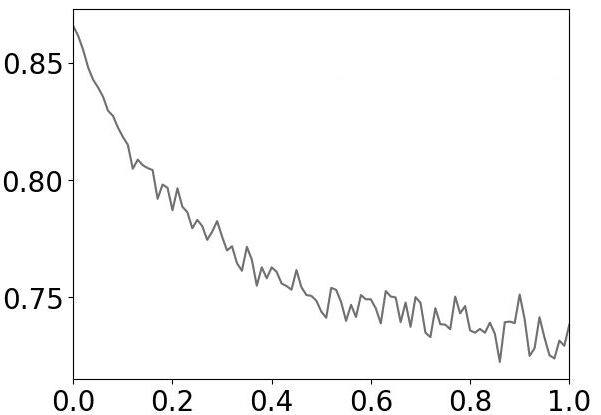
\includegraphics[width=0.48\textwidth]{media/From_IEEE/res_elec_100_h_10_rerun.csv_F1_score_reduced.jpg}
         \label{fig:f1_elec}}
    \subfloat[]{
         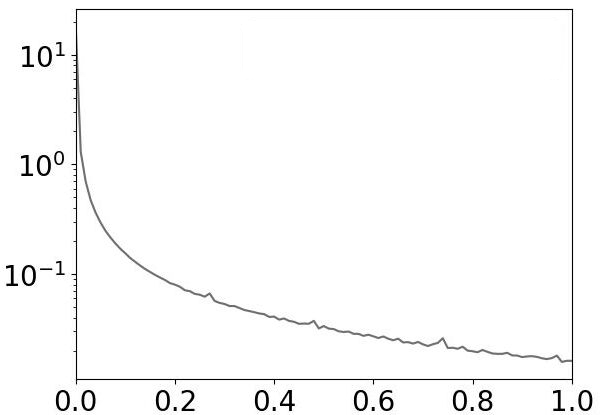
\includegraphics[width=0.48\textwidth]{media/From_IEEE/res_elec_100_h_10_rerun.csv_iter_time_reduced.jpg}
         \label{fig:iter_elec}}
    \\
    \subfloat[]{
         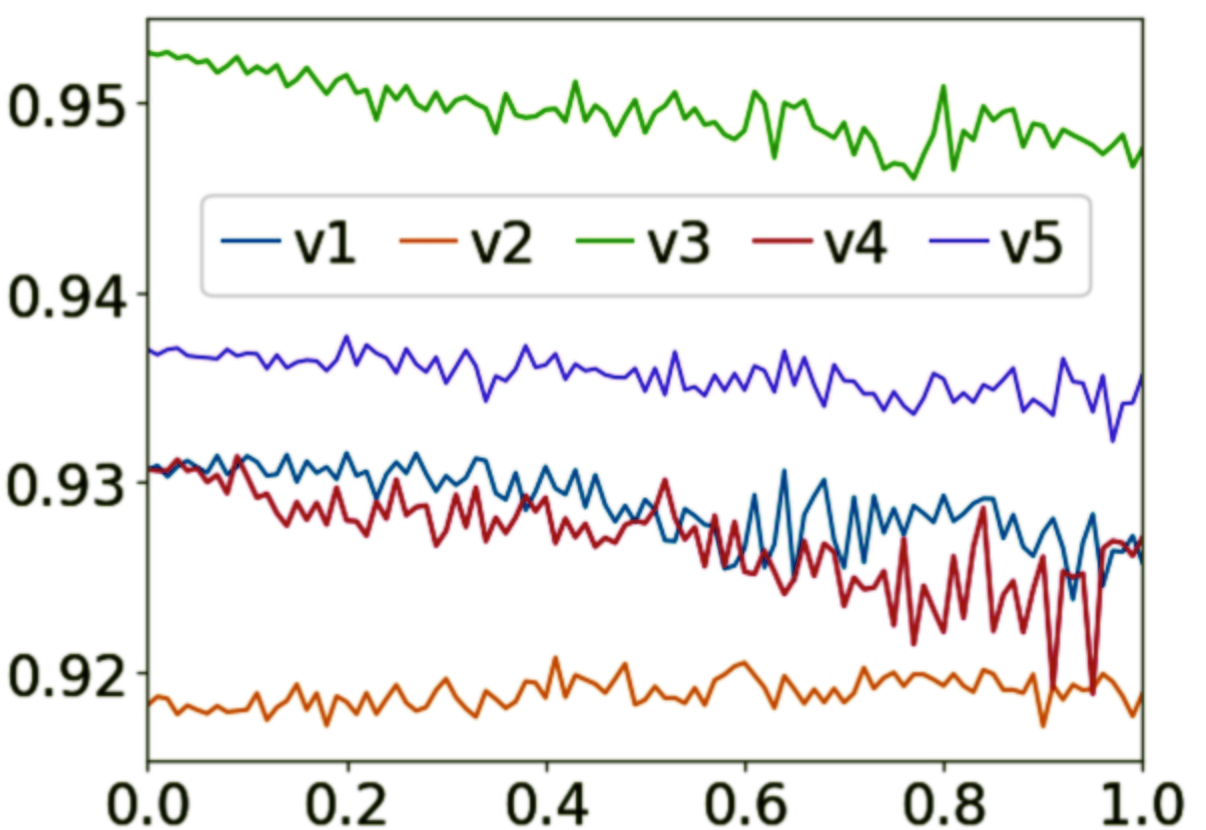
\includegraphics[width=0.48\textwidth]{media/From_IEEE/INSECTS-aggregated_3_F1_score.jpg}
         \label{fig:f1_insects}}
    \subfloat[]{
         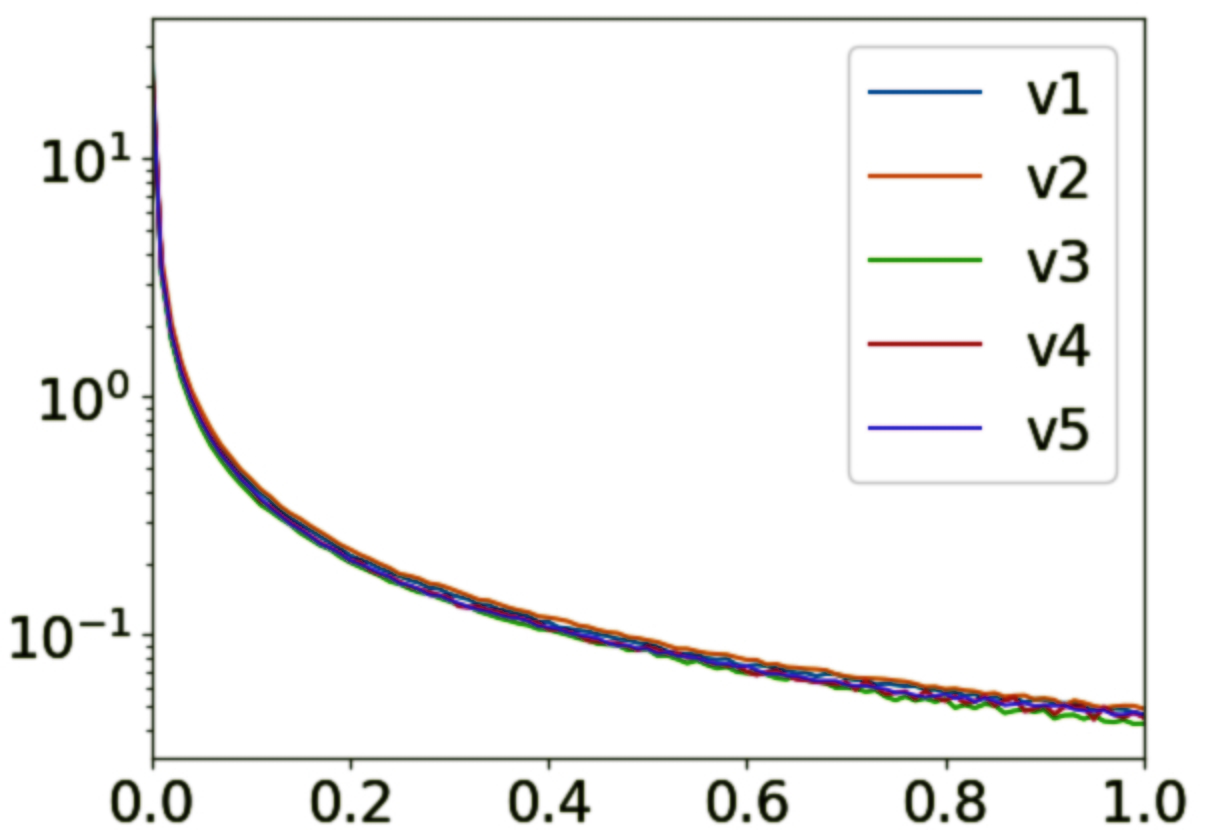
\includegraphics[width=0.48\textwidth]{media/From_IEEE/INSECTS-aggregated_3_iter_time_reduced.jpg}
         \label{fig:iter_insects}}
    \\
    \subfloat[]{
         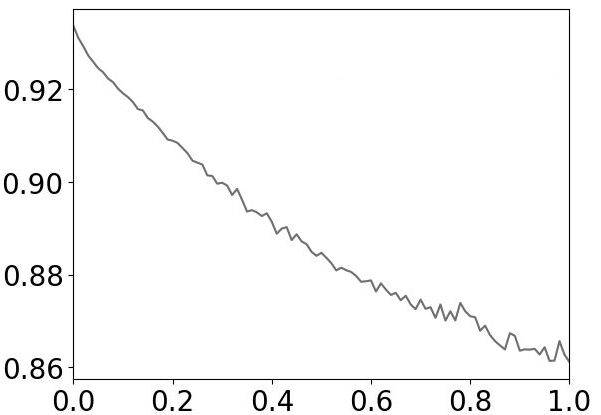
\includegraphics[width=0.48\textwidth]{media/From_IEEE/res_poker-lsn_1000_h_10.csv_F1_score_reduced.jpg}
         \label{fig:f1_poker}}
    \subfloat[]{
         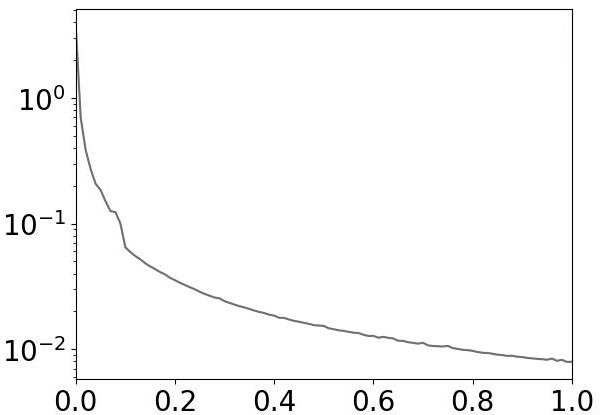
\includegraphics[width=0.48\textwidth]{media/From_IEEE/res_poker-lsn_1000_h_10.csv_iter_time_reduced.jpg}
         \label{fig:iter_poker}}
\caption{Performance of \algo\ in the SW model on the Electricity, INSECTS and Poker datasets (top to bottom), in terms of F1-score (left) and amortized milliseconds per update (right) as a function of $\epsilon$.}\label{fig:SW}
\vspace*{10pt}
\end{figure}

\begin{figure}
\vspace*{10pt}
    \centering
    \subfloat[]{
         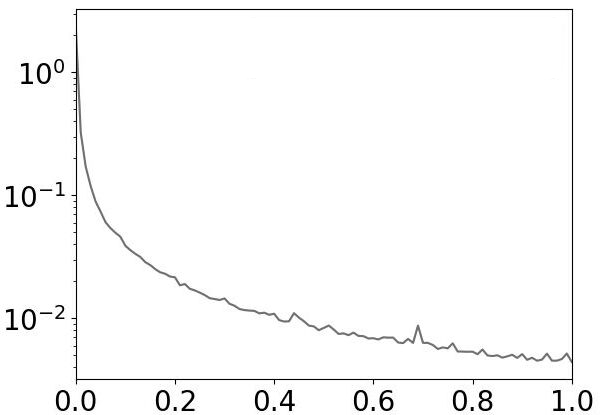
\includegraphics[width=0.5\textwidth]{media/From_IEEE/elec_random.csv_iter_time_reduced.jpg}
         \label{fig:ru_elec}    
    }
    \hfill
    \subfloat[]{
         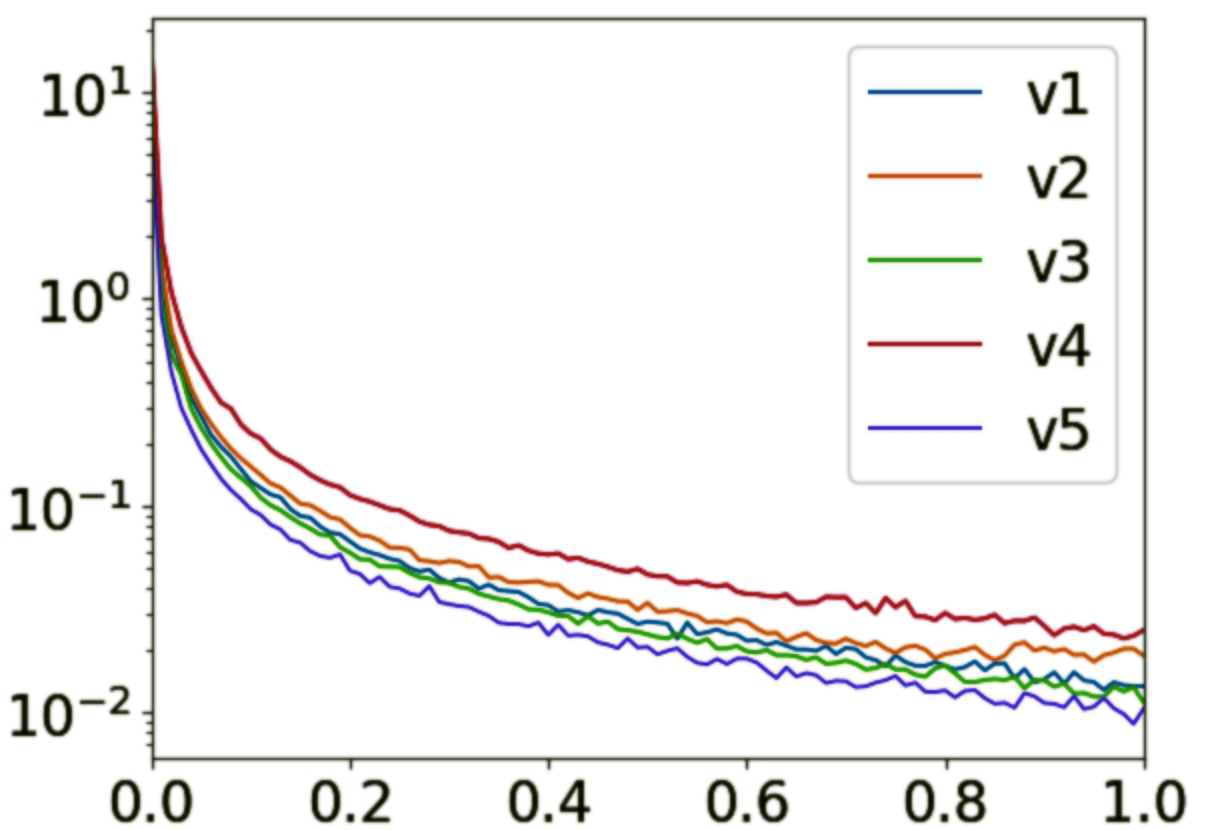
\includegraphics[width=0.5\textwidth]{media/From_IEEE/INSECTS_random-aggregated_3_iter_time_reduced.jpg}
         \label{fig:ru_insects}    
    }
    % \\[15pt]
    % \subfloat[]{
    %      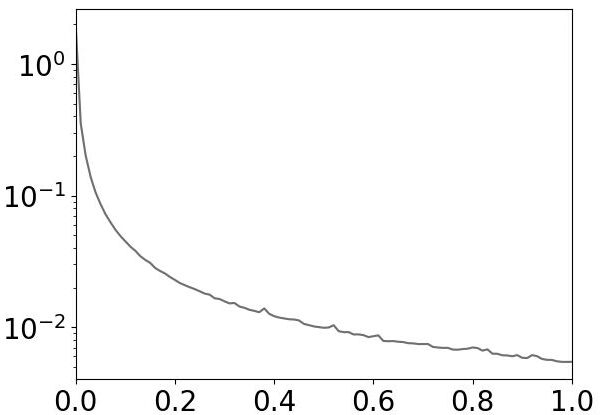
\includegraphics[width=0.5\textwidth]{media/From_IEEE/poker-lsn_random.csv_iter_time_reduced.jpg}
    %      \label{fig:ru_poker}    
    % }
%\caption{Amortized running time of \algo\ in the RU model on the Electricity (left) and INSECTS (right) datasets. Amortized running time for the Poker dataset is very similar to Electricity.}

\caption{Amortized running time per update (in milliseconds) of \algo\ in the RU model on the Electricity (left) and INSECTS (right) datasets. The Poker dataset yields similar results.}

\label{fig:RU}
\end{figure}




\iffalse
\begin{figure*}
    \centering
    \subfloat[Electricity (F1-score)]{
         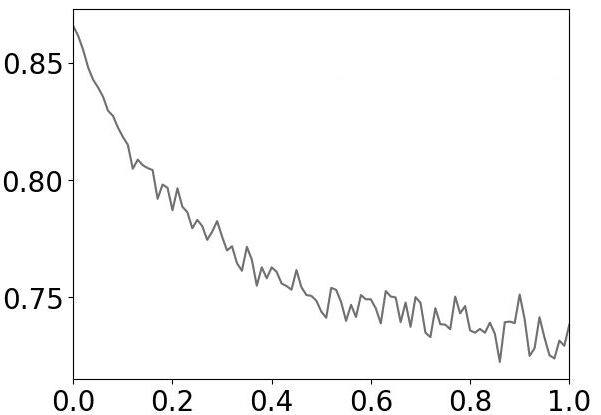
\includegraphics[width=0.3\textwidth]{media/From_IEEE/res_elec_100_h_10_rerun.csv_F1_score_reduced.jpg}
         \label{fig:f1_elec}}
    \hfill
    \subfloat[INSECTS (F1-score)]{
         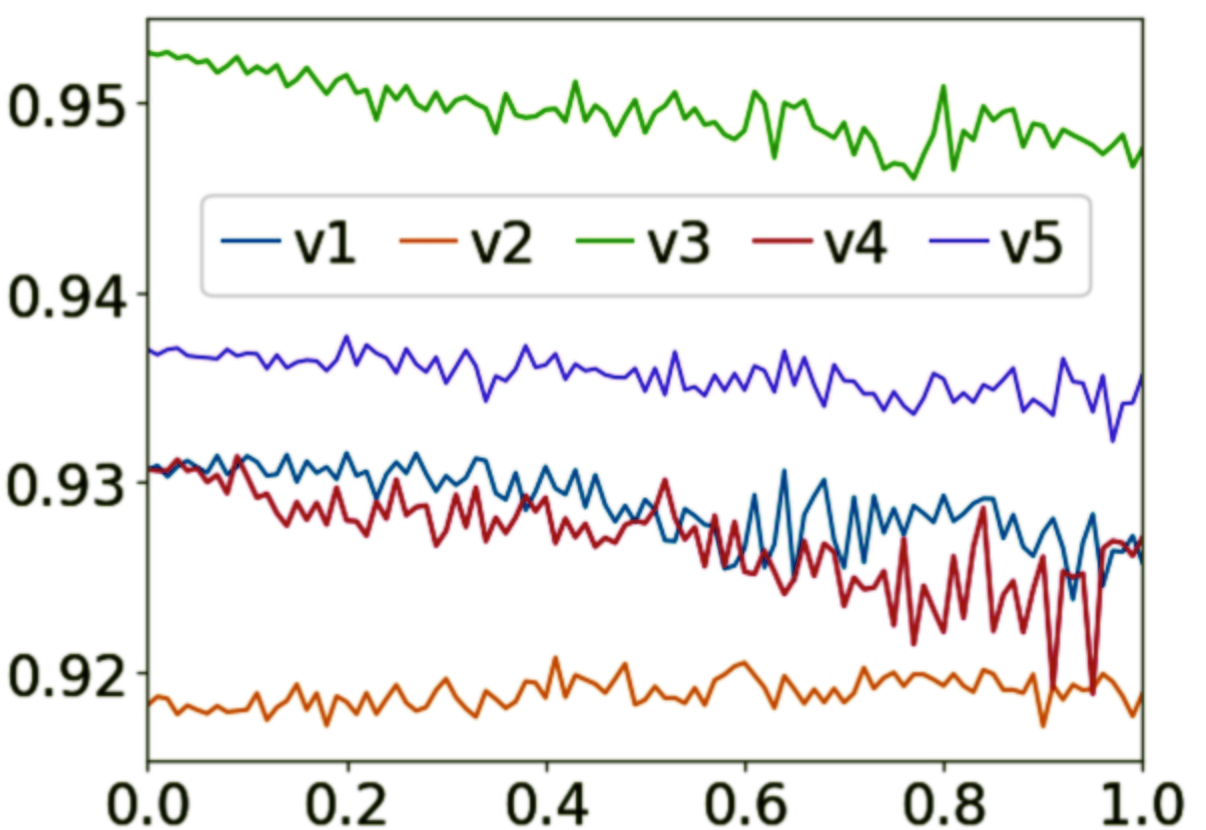
\includegraphics[width=0.28\textwidth]{media/From_IEEE/INSECTS-aggregated_3_F1_score.jpg}
         \label{fig:f1_insects}}
    \hfill
    \subfloat[Poker (F1-score)]{
         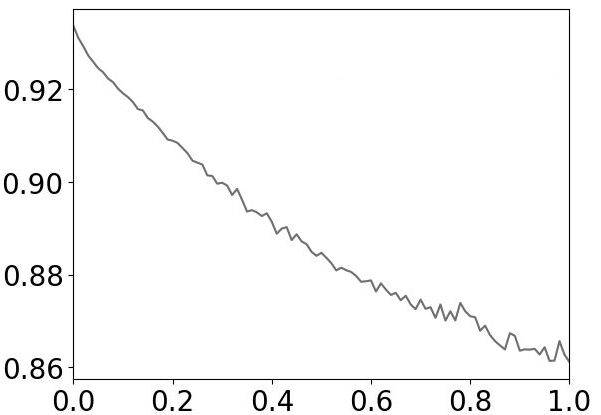
\includegraphics[width=0.3\textwidth]{media/From_IEEE/res_poker-lsn_1000_h_10.csv_F1_score_reduced.jpg}
         \label{fig:f1_poker}    
    }
    \label{fig:f1_scores}
    \subfloat[Electricity (Time)]{
         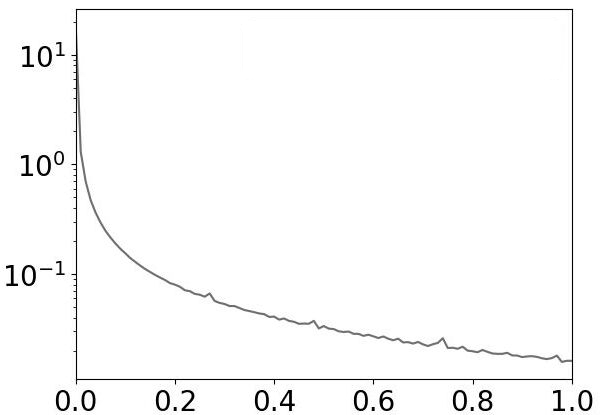
\includegraphics[width=0.3\textwidth]{media/From_IEEE/res_elec_100_h_10_rerun.csv_iter_time_reduced.jpg}
         \label{fig:iter_elec}    
    }
    \hfill
        \subfloat["INSECTS" (Time)]{
         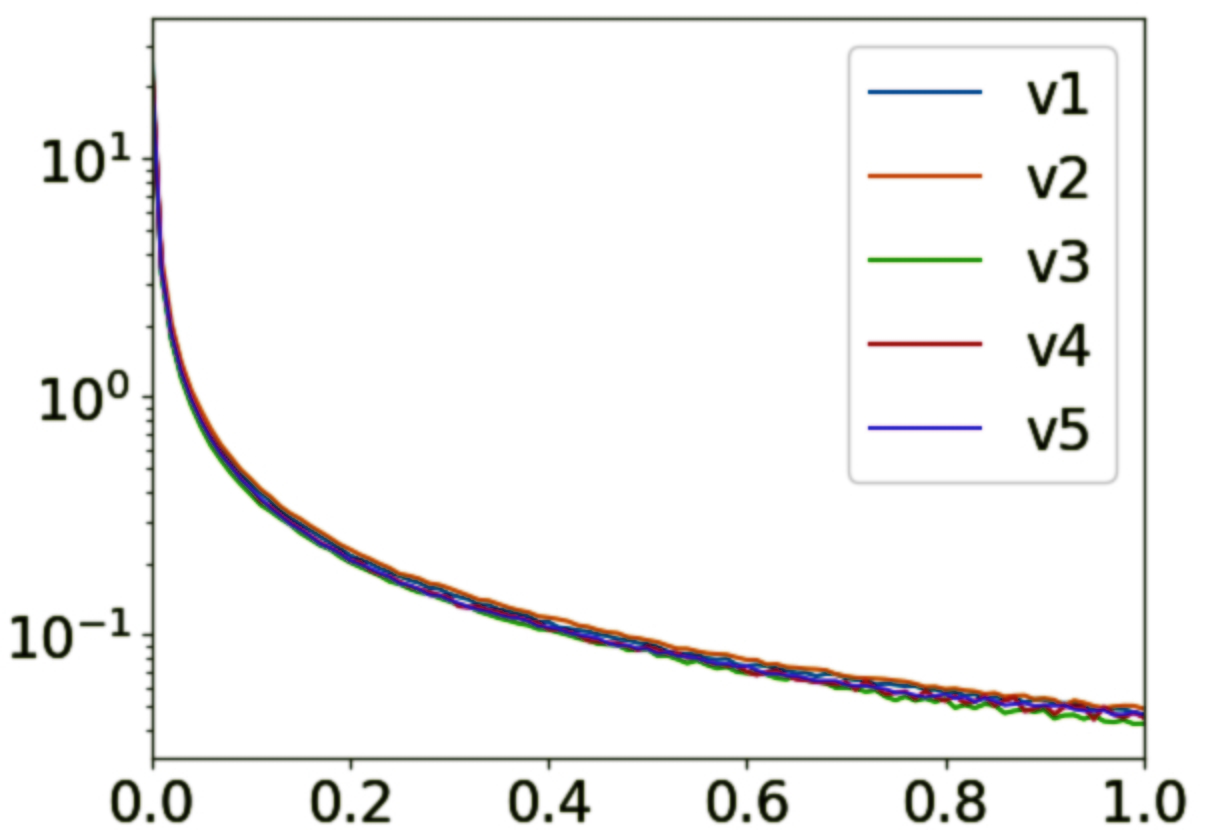
\includegraphics[width=0.28\textwidth]{media/From_IEEE/INSECTS-aggregated_3_iter_time_reduced.jpg}
         \label{fig:iter_insects}    
    }
    \hfill
    \subfloat[Poker (Time)]{
         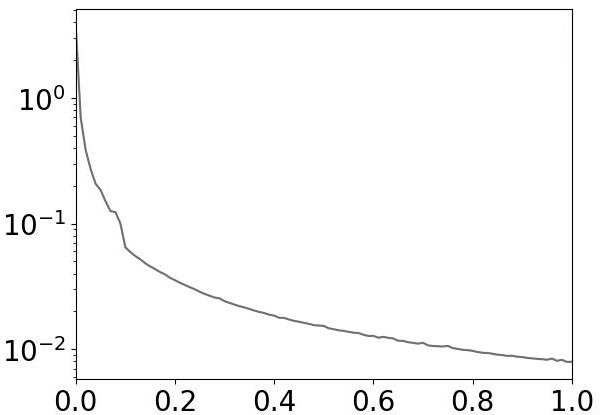
\includegraphics[width=0.3\textwidth]{media/From_IEEE/res_poker-lsn_1000_h_10.csv_iter_time_reduced.jpg}
         \label{fig:iter_poker}    
    }
\caption{F1-score and amortized running time in the SW model.}\label{fig:SW}

\end{figure*}
\fi

\iffalse
\begin{figure*}
    \centering
    \subfloat[Electricity]{
         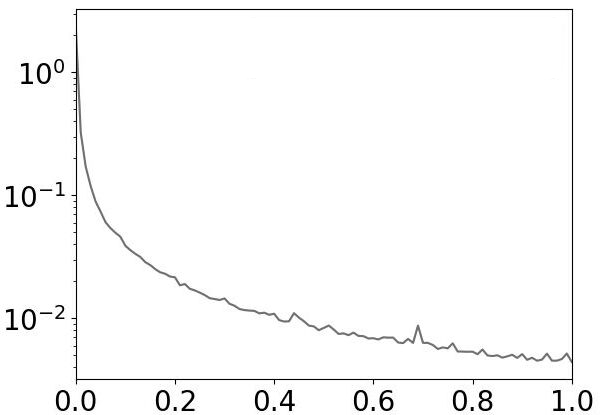
\includegraphics[width=0.3\textwidth]{media/From_IEEE/elec_random.csv_iter_time_reduced.jpg}
         \label{fig:ru_elec}    
    }
    \hfill
    \subfloat[INSECTS]{
         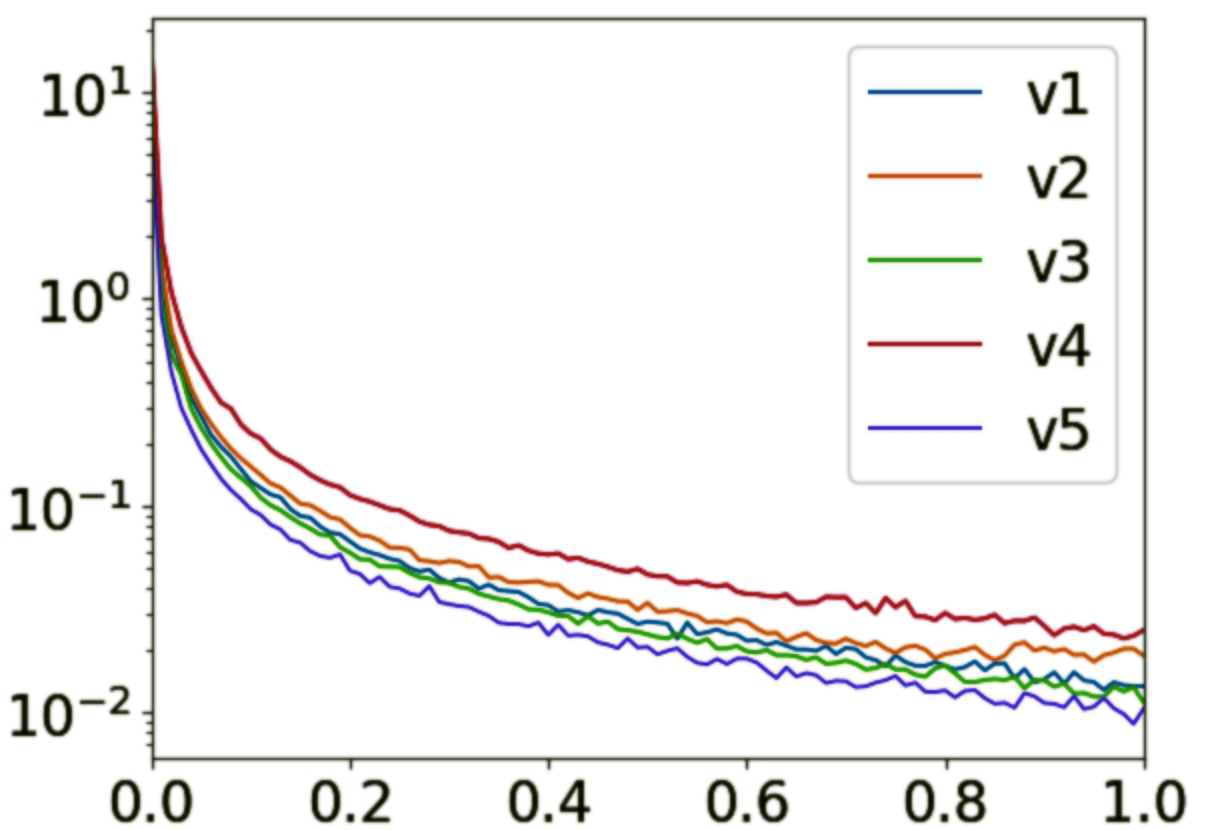
\includegraphics[width=0.28\textwidth]{media/From_IEEE/INSECTS_random-aggregated_3_iter_time_reduced.jpg}
         \label{fig:ru_insects}    
    }
    \hfill
    \subfloat[Poker]{
         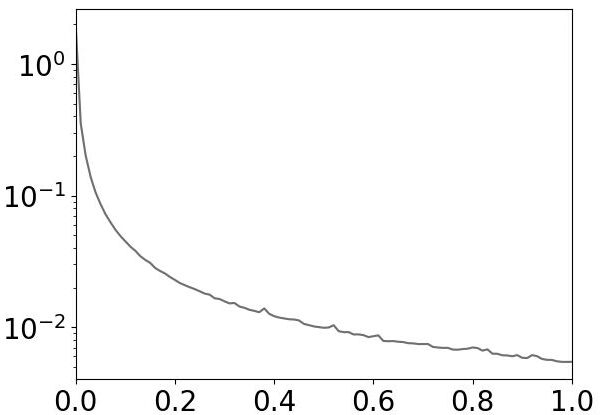
\includegraphics[width=0.3\textwidth]{media/From_IEEE/poker-lsn_random.csv_iter_time_reduced.jpg}
         \label{fig:ru_poker}    
    }
\caption{Amortized running time in the RU model.}\label{fig:RU}
\end{figure*}
\fi

%\iffalse
\subsection{Conclusions and Future Work}
We developed the first fully dynamic algorithm for maintaining $\epsilon$-feasible decision trees, while we proved it to be nearly optimal in terms of space and amortized time. Our work shows that many well-known decision tree algorithms, whether offline like CART or incremental like EDFT, can be made fully dynamic with a small loss in the quality of the decision tree and a small overhead in the amortized running time. Our work leaves open the natural question of whether these results can be strengthened from amortized to worst-case. We believe this is an exciting direction for future research in  fully-dynamic supervised machine learning.
%We developed the first fully dynamic algorithm for maintaining $\epsilon$-feasible decision trees, as well as lower bounds on the space requirements and amortized running time of any such algorithm. Our algorithm boasts near-optimal space requirements and near-optimal running time for some cases of interest. Our experimental evaluation shows that our algorithm is accurate in terms of F1-score, while boasting an average running per update of less than one millisecond. We believe that developing fully-dynamic algorithms for supervised machine learning problems is an exciting research direction that deserves more attention. 
%\fi